
%% LyX 2.2.1 created this file.  For more info, see http://www.lyx.org/.
%% Do not edit unless you really know what you are doing.
\documentclass[11pt]{beamer}\usepackage[]{graphicx}\usepackage[]{color}
% maxwidth is the original width if it is less than linewidth
% otherwise use linewidth (to make sure the graphics do not exceed the margin)
\makeatletter
\def\maxwidth{ %
  \ifdim\Gin@nat@width>\linewidth
    \linewidth
  \else
    \Gin@nat@width
  \fi
}
\makeatother

\definecolor{fgcolor}{rgb}{0.345, 0.345, 0.345}
\newcommand{\hlnum}[1]{\textcolor[rgb]{0.686,0.059,0.569}{#1}}%
\newcommand{\hlstr}[1]{\textcolor[rgb]{0.192,0.494,0.8}{#1}}%
\newcommand{\hlcom}[1]{\textcolor[rgb]{0.678,0.584,0.686}{\textit{#1}}}%
\newcommand{\hlopt}[1]{\textcolor[rgb]{0,0,0}{#1}}%
\newcommand{\hlstd}[1]{\textcolor[rgb]{0.345,0.345,0.345}{#1}}%
\newcommand{\hlkwa}[1]{\textcolor[rgb]{0.161,0.373,0.58}{\textbf{#1}}}%
\newcommand{\hlkwb}[1]{\textcolor[rgb]{0.69,0.353,0.396}{#1}}%
\newcommand{\hlkwc}[1]{\textcolor[rgb]{0.333,0.667,0.333}{#1}}%
\newcommand{\hlkwd}[1]{\textcolor[rgb]{0.737,0.353,0.396}{\textbf{#1}}}%
\let\hlipl\hlkwb

\usepackage{framed}
\makeatletter
\newenvironment{kframe}{%
 \def\at@end@of@kframe{}%
 \ifinner\ifhmode%
  \def\at@end@of@kframe{\end{minipage}}%
  \begin{minipage}{\columnwidth}%
 \fi\fi%
 \def\FrameCommand##1{\hskip\@totalleftmargin \hskip-\fboxsep
 \colorbox{shadecolor}{##1}\hskip-\fboxsep
     % There is no \\@totalrightmargin, so:
     \hskip-\linewidth \hskip-\@totalleftmargin \hskip\columnwidth}%
 \MakeFramed {\advance\hsize-\width
   \@totalleftmargin\z@ \linewidth\hsize
   \@setminipage}}%
 {\par\unskip\endMakeFramed%
 \at@end@of@kframe}
\makeatother

\definecolor{shadecolor}{rgb}{.97, .97, .97}
\definecolor{messagecolor}{rgb}{0, 0, 0}
\definecolor{warningcolor}{rgb}{1, 0, 1}
\definecolor{errorcolor}{rgb}{1, 0, 0}
\newenvironment{knitrout}{}{} % an empty environment to be redefined in TeX

\usepackage{alltt}
\usepackage[T1]{fontenc}
\usepackage[utf8]{inputenc}
\setcounter{secnumdepth}{3}
\setcounter{tocdepth}{3}
\usepackage{url}
\ifx\hypersetup\undefined
  \AtBeginDocument{%
    \hypersetup{unicode=true,pdfusetitle,
 bookmarks=true,bookmarksnumbered=false,bookmarksopen=false,
 breaklinks=false,pdfborder={0 0 0},pdfborderstyle={},backref=false,colorlinks=false}
  }
\else
  \hypersetup{unicode=true,pdfusetitle,
 bookmarks=true,bookmarksnumbered=false,bookmarksopen=false,
 breaklinks=false,pdfborder={0 0 0},pdfborderstyle={},backref=false,colorlinks=false}
\fi
\usepackage{breakurl}

\makeatletter

%%%%%%%%%%%%%%%%%%%%%%%%%%%%%% LyX specific LaTeX commands.
\providecommand{\LyX}{\texorpdfstring%
  {L\kern-.1667em\lower.25em\hbox{Y}\kern-.125emX\@}
  {LyX}}

%%%%%%%%%%%%%%%%%%%%%%%%%%%%%% Textclass specific LaTeX commands.
 % this default might be overridden by plain title style
 \newcommand\makebeamertitle{\frame{\maketitle}}%
 % (ERT) argument for the TOC
 \AtBeginDocument{%
   \let\origtableofcontents=\tableofcontents
   \def\tableofcontents{\@ifnextchar[{\origtableofcontents}{\gobbletableofcontents}}
   \def\gobbletableofcontents#1{\origtableofcontents}
 }
 
 \renewenvironment{knitrout}{\setlength{\topsep}{0mm}}{} 

%%%%%%%%%%%%%%%%%%%%%%%%%%%%%% User specified LaTeX commands.
\usetheme{default}

\makeatother

 \usepackage[utf8]{inputenc}
\usepackage[T1]{fontenc}
\usepackage[english]{babel}

%\usepackage{verbatim}

\usepackage[export]{adjustbox}

\usepackage{
    amsmath,
    amsfonts,
    etex,
    fancyvrb,
    graphicx,
    multicol,
    pifont,
    setspace,
    soul,
    spverbatim,
    textcomp,
    xcolor,
    xspace
}

\usepackage{tikz}
\usetikzlibrary{shadows}

%%%SETUP%%%
\hypersetup{
     colorlinks = true,
     linkcolor = blue,
     anchorcolor = blue,
     citecolor = blue,
     filecolor = blue,
     urlcolor = blue
     }
     
%%%THEOREMS%%%
\theoremstyle{example}
\newtheorem*{exercise}{Exercise}
\newtheorem*{question}{Question}
\newtheorem*{answer}{\emph{Answer}}
\newtheorem*{notation}{Notation}

%%%TWEAKS%%%
\setlength\arraycolsep{4pt}
\addtolength\fboxsep{10pt}
\setstretch{1.4}
\setbeamersize{description width=3em}
\setbeamersize{text margin left=.5cm,text margin right=.5cm} 
\renewcommand{\emph}{\alert}
\renewcommand{\arraystretch}{1.2}
\renewcommand{\tabcolsep}{4pt}
\setbeamercolor{alerted text}{fg=magenta}


\graphicspath{{img/}}

%for straight quotes in verbatim:
\usepackage{upquote,textcomp}

%turn off navigation symbols
\beamertemplatenavigationsymbolsempty
\setbeamertemplate{footline}[frame number]

%title page

\author
  [Dr.\ Irene Vrbik]
  {Dr.\ Irene Vrbik}

\date
  {}

\institute
  {University of British Columbia Okanagan \newline \texttt{irene.vrbik@ubc.ca}}
  
 \definecolor{iyellow}{RGB}{255, 162, 23}
\definecolor{sgreen}{RGB}{118, 191, 138}

\newcommand{\yellow}[1]{\textcolor{iyellow}{#1}}
\newcommand{\red}[1]{\textcolor{red}{#1}}
\newcommand{\green}[1]{\textcolor{ForestGreen}{#1}}
\newcommand{\blue}[1]{{\textcolor{blue}{#1}}}
\newcommand{\orange}[1]{{\textcolor{orange}{#1}}}
\newcommand{\bblue}[1]{\textcolor{SteelBlue!90!gray}{#1}} % beamer blue
\newcommand{\purple}[1]{{\textcolor{purple}{#1}}}

\newcommand{\el}{\\[1em]\pause}
\newcommand{\nl}{\\[1em]}
\newcommand{\define}[1]{\textbf{\textcolor{orange}{#1}}}

%\newcommand{\answer}[1]{\textit{\textbf{\textcolor{iyellow}{#1}}}}

\newcommand{\command}[1]{\texttt{\textbf{\textcolor{DarkMagenta}{#1}}}}
\newcommand{\ipic}[2]{\includegraphics[width={#2}\textwidth]{#1}}
\newcommand{\cell}[1]{{\sf \textbf{\textcolor{DarkMagenta}{#1}}}}
\newcommand{\ra}{$\rightarrow$}

\newcommand{\ft}[1]{\frametitle{#1}}


\newenvironment{allintypewriter}{\ttfamily}{\par}
\newcommand{\bs}{$\backslash$}

\newcommand*\keystroke[1]{%
  \tikz[baseline=(key.base)]
    \node[%
      draw,
      fill=white,
      drop shadow={shadow xshift=0.25ex,shadow yshift=-0.25ex,fill=black,opacity=0.75},
      rectangle,
      rounded corners=2pt,
      inner sep=1pt,
      line width=0.5pt,
      font=\scriptsize\sffamily
    ](key) {#1\strut}
  ;
}

% timed answer
\newcommand{\tans}[2]{\textbf<#1>{\textit<#1>{{\color<#1>{iyellow}{#2}}}}}


\makeatletter
\g@addto@macro\normalsize{%
  \setlength\abovedisplayskip{0.4em}
  \setlength\belowdisplayskip{0.4em}
  \setlength\abovedisplayshortskip{0.2em}
  \setlength\belowdisplayshortskip{0.2em}
}
\makeatother


\newcommand{\cmark}{{\Large\color{green}\ding{51}}}%
\newcommand{\xmark}{{\Large\color{red}\ding{55}}}%

\newcommand{\pcmark}{\onslide<+->{\cmark}}
\newcommand{\pxmark}{\onslide<+->{\xmark}}

\newcommand{\by}{\overline{y}}
\newcommand{\ty}{\tilde{y}}
\IfFileExists{upquote.sty}{\usepackage{upquote}}{}
\begin{document}


\title[Data 301]{An Introduction to \R and \RStudio}

\makebeamertitle


\section{RStudio}

%%%%%%%%%%%%%%%%%%%%%%%%%%%%%%%%%%%%%%%%%%%%%%%%%%%%%%%%%%%%%%%%%%%%%%%%%%%%%%%%%%%%%%%%%%%%%%%%%%%%
\begin{frame}{What is R?}

\begin{itemize}
\item R is a free and open source programming language for statistical computing and graphics.\nl
\item It is one of the most widely used programming languages for statistical analysis.\nl
\item R is popular in both in academia and industry:
\begin{description}
% \item [Facebook] For behavior analysis related to status updates and profile pictures.
\item [Google] For advertising effectiveness and economic forecasting.
\item [Twitter] For data visualization and semantic clustering
% \item[Microsoft] Acquired Revolution R company and use it for a variety of purposes.
\item[Uber] For statistical analysis
\end{description}
see \href{https://www.listendata.com/2016/12/companies-using-r.html}{here} for a full list of companies using R. 
\end{itemize}
\end{frame}
%%%%%%%%%%%%%%%%%%%%%%%%%%%%%%%%%%%%%%%%%%%%%%%%%%%%%%%%%%%%%%%%%%%%%%%%%%%%%%%%%%%%%%%%%%%%%%%%%%%



\begin{frame}[fragile]{Why learn R? }
\begin{itemize}
\item One major attraction of {\tt R} is its rich variety of libraries.
\item New libraries/packages (akin to Python modules) are continuously being added to the official open-source repository called \href{https://cran.r-project.org/}{CRAN} (Comprehensive R Archive Network).
\item There currently over \href{https://blog.revolutionanalytics.com/2017/01/cran-10000.html}{12000} packages which you can see by name  \href{cran.r-project.org/web/packages/available_packages_by_name.html}{here}.
% \item Chances are, if you have a problem that needs solving, there is a package that will help you g 
\item In addition, mathematical calculations (eg vector operations, matrix multiplication) can be done in base R (i.e. without having to install any pacakges). 
% Common mathematical operations like matrix multiplication work straight out of the box, and the language’s array-oriented syntax makes it easier to translate from math to code, especially for someone with no or minimal programming background.
% \item R creates high quality graphs and visualizations.
\end{itemize}
\end{frame}



\begin{frame}[fragile]{R vs. Python}
% https://blog.udacity.com/2015/01/python-vs-r-learn-first.html
% https://www.datacamp.com/community/tutorials/r-or-python-for-data-analysis
% https://www.guru99.com/r-vs-python.html
\begin{itemize}
\item Both Python and R are amongst the most popular languages for data analysis.
\item While Python may be touted as a more general-purpose languages, {\tt R} has been targeted towards for statisticians and data scientist.
% designed to answer statistical problems, machine learning, and data science.
\item {\tt R} therefore does much of the heavy lifting in terms of analysis and graphing.
\item Here are some interesting articles comparing Python to {\tt R}: \href{https://www.guru99.com/r-vs-python.html}{guru99}, \href{https://www.datacamp.com/community/tutorials/r-or-python-for-data-analysis}{datacamp}, \href{https://towardsdatascience.com/data-science-101-is-python-better-than-r-b8f258f57b0f}{towardsdatascience}.
%While Python is often praised for being a general-purpose language with an easy-to-understand syntax, R's functionality is developed with statisticians in mind, thereby giving it field-specific advantages such as great features for data visualization.
\end{itemize}
\end{frame}



%%%%%%%%%%%%%%%%%%%%%%%%%%%%%%%%%%%%%%%%%%%%%%%%%%%%%%%%%%%%%%%%%%%%%%%%%%%%%%%%%%%%%%%%%%%%%%%%%%%%
\begin{frame}[fragile]
\begin{example}
Filtering a dataset to be within a lower and upper bound and then calculating summary statistics.\\[2em]

\begin{Verbatim}[xleftmargin=2em, xrightmargin=1.5em, frame=single, numbers=left, label=Python, framesep=0.5em]
for v in data:
    if lower <= v <= upper:
        maxdata = max(v, maxdata)
        mindata = min(v, mindata)
    sumdata += v
    count += 1
\end{Verbatim}
\end{example}
\end{frame}
%%%%%%%%%%%%%%%%
%manual uncover%
%%%%%%%%%%%%%%%%
\begin{frame}[fragile]
\begin{example}
Filtering a dataset to be within a lower and upper bound and then calculating summary statistics.\\[2em]

\begin{Verbatim}[xleftmargin=2em, xrightmargin=1.5em, frame=single, numbers=left, label=R, framesep=0.5em]
new_data <- subset(data, x <= upper & x >= lower)
sumdata <- sum(new_data)
count <- length(new_data)
maxdata <- max(new_data)
mindata <- min(new_data)
\end{Verbatim}
\end{example}
\end{frame}
%%%%%%%%%%%%%%

\begin{frame}[fragile]{Statistics Review: Types of Data}
Before diving into the R specifics, a brief review of some topics in statistics are in order.  Recall that we can generalize data into two types:
\begin{enumerate}
  \item Qualitative (Categorical)
    \begin{enumerate}
      \item Descriptions or groups
      \item Can be characters or numbers
      \item Observed and not measured
      \item i.e. names, labels, categories, properties
    \end{enumerate}
%
  \item Quantitative (Numeric)
    \begin{enumerate}
      \item Strictly numeric
      \item Can be measured
      \item i.e. height, weight, speed, counts, temperature, volume
    \end{enumerate}
\end{enumerate}
\end{frame}
%%%%%%%%%%%%%%%%%%%%%%%%%%%%%%%%%%%%%%%%%%%%%%%%%%%%%%%%%%%%%%%%%%%%%%%%%%%%%%%%%%%%%%%%%%%%%%%%%%%%


%%%%%%%%%%%%%%%%%%%%%%%%%%%%%%%%%%%%%%%%%%%%%%%%%%%%%%%%%%%%%%%%%%%%%%%%%%%%%%%%%%%%%%%%%%%%%%%%%%%%
\begin{frame}[fragile]{Summaries of Data}
\begin{itemize}
\item A \emph{numerical summary} provides an overview of data to help understand it without examining all data values.
\vfill
\item A \emph{measure of centre} and a \emph{measure of spread} to describe quantitative data. \vfill
\item There are no numerical summaries for qualitative data, only \emph{graphical summaries}. 
\vfill
\end{itemize}
\end{frame}
%%%%%%%%%%%%%%%%%%%%%%%%%%%%%%%%%%%%%%%%%%%%%%%%%%%%%%%%%%%%%%%%%%%%%%%%%%%%%%%%%%%%%%%%%%%%%%%%%%%%


%%%%%%%%%%%%%%%%%%%%%%%%%%%%%%%%%%%%%%%%%%%%%%%%%%%%%%%%%%%%%%%%%%%%%%%%%%%%%%%%%%%%%%%%%%%%%%%%%%%%
\begin{frame}[fragile]{Measures of Centre}
\begin{definition}[Mean]
The \emph{mean} is the average of data values (sum of values divided by count):
$$
\by = \frac{\sum_{i=1}^n y_i}{n}
$$
\end{definition}

\begin{definition}[Median]
The \emph{median} is the value at which half of the data lies above that value and half lies below it.
\begin{enumerate}
\item Odd number of observations: $\ty$ is the $k$th value where $k = \frac{n+1}2$.
\item Even number of observations: $\ty$ is the mean of the $k$th and $(k+1)$ terms, where $k = \frac n 2$.
\end{enumerate}
\end{definition}
\end{frame}
%%%%%%%%%%%%%%%%%%%%%%%%%%%%%%%%%%%%%%%%%%%%%%%%%%%%%%%%%%%%%%%%%%%%%%%%%%%%%%%%%%%%%%%%%%%%%%%%%%%%


%%%%%%%%%%%%%%%%%%%%%%%%%%%%%%%%%%%%%%%%%%%%%%%%%%%%%%%%%%%%%%%%%%%%%%%%%%%%%%%%%%%%%%%%%%%%%%%%%%%%
\begin{frame}[fragile]
\begin{example}
Let the data be given by $y = \{1,\, 3,\, 3,\, 7,\, 9 \}$.  The \emph{mean} is
$$\by = \frac{1 + 3 + 3 + 7 + 9}{5} = 4.6$$
and the \emph{median} is
$$\ty = 3$$
for which R provides \texttt{mean()} and \texttt{median()}:
\begin{Verbatim}[commandchars=\\\{\}, xleftmargin=2em]
\emph{> mean(y)}
[1] 4.6
\emph{> median(y)}
[1] 3
\end{Verbatim}
\end{example}
\end{frame}
%%%%%%%%%%%%%%%%%%%%%%%%%%%%%%%%%%%%%%%%%%%%%%%%%%%%%%%%%%%%%%%%%%%%%%%%%%%%%%%%%%%%%%%%%%%%%%%%%%%%


%%%%%%%%%%%%%%%%%%%%%%%%%%%%%%%%%%%%%%%%%%%%%%%%%%%%%%%%%%%%%%%%%%%%%%%%%%%%%%%%%%%%%%%%%%%%%%%%%%%%
\begin{frame}[fragile]{Measures of Spread}
A measure of spread indicates how far apart the values are.
\begin{definition}[Variance]
\emph{Variance} is the sum of the squares of each data point's distance from the mean:
$$s^2 = \frac{\sum_{i=1}^n (y_i-\by)^2}{n-1} = \frac{\sum_{i=1}^n y_i^2 - n\by^2}{n-1}$$
\end{definition}

\begin{definition}[Standard Deviation]
\emph{Standard Deviation} is the square root of the variance: $s = \sqrt{s^2}$
\end{definition}

\begin{definition}[Range]
\emph{Range} is the maximum value minus minimum value: $\max(y) - \min(y)$.
\end{definition}
\end{frame}
%%%%%%%%%%%%%%%%%%%%%%%%%%%%%%%%%%%%%%%%%%%%%%%%%%%%%%%%%%%%%%%%%%%%%%%%%%%%%%%%%%%%%%%%%%%%%%%%%%%%


%%%%%%%%%%%%%%%%%%%%%%%%%%%%%%%%%%%%%%%%%%%%%%%%%%%%%%%%%%%%%%%%%%%%%%%%%%%%%%%%%%%%%%%%%%%%%%%%%%%%
\begin{frame}[fragile]
\begin{example}[Standard Deviation]
Let $y = (1, 3, ,3,7, 9)$ then the \emph{variance} is
$$s^2 = \frac{(1+9+9+49+81)-(5 \cdot 4.6^2)}{5-1} = 10.8$$
and therefore the \emph{standard deviation is}
$$s = 3.286$$
for which R provides \texttt{mean()} and \texttt{median()}:
\begin{Verbatim}[commandchars=\\\{\}, xleftmargin=2em]
\emph{> var(y)}
[1] 10.8
\emph{> median(y)}
[1] 3.286335
\end{Verbatim}
\end{example}
\end{frame}
%%%%%%%%%%%%%%%%%%%%%%%%%%%%%%%%%%%%%%%%%%%%%%%%%%%%%%%%%%%%%%%%%%%%%%%%%%%%%%%%%%%%%%%%%%%%%%%%%%%%


%%%%%%%%%%%%%%%%%%%%%%%%%%%%%%%%%%%%%%%%%%%%%%%%%%%%%%%%%%%%%%%%%%%%%%%%%%%%%%%%%%%%%%%%%%%%%%%%%%%%
\begin{frame}[fragile]
\begin{question}
Let $y = (1, 3, 4, 7, 11, 28)$.  How many of the are following statements are true?
\begin{enumerate}
\item $\by = \ty$
\item $\by = 9$
\item $s^2 = 3.5$
\item ${\rm range} = 6$. 
\end{enumerate}
\end{question}
\begin{multicols}{5}
\begin{enumerate}[A)]
\item 0
\item 1
\item 2
\item 3
\item 4
\end{enumerate}
\end{multicols}
\end{frame}


\begin{frame}<handout:0>[fragile]
\begin{question}
Let $y = (1, 3, 4, 7, 11, 28)$.  How many of the are following statements are true?
\begin{enumerate}
\item $\by = \ty$, \onslide<+->{}\pxmark
\item $\by = 9$, \pcmark
\item $s^2 = 3.5$, \pxmark
\item ${\rm range} = 6$. \pxmark
\end{enumerate}
\begin{multicols}{5}
\begin{enumerate}[A)]
\item 0
\item 1
\item \tans{5}{2}
\item 3
\item 4
\end{enumerate}
\end{multicols}
\end{question}
\end{frame}
%%%%%%%%%%%%%%%%%%%%%%%%%%%%%%%%%%%%%%%%%%%%%%%%%%%%%%%%%%%%%%%%%%%%%%%%%%%%%%%%%%



%%%%%%%%%%%%%%%%%%%%%%%%%%%%%%%%%%%%%%%%%%%%%%%%%%%%%%%%%%%%%%%%%%%%%%%%%%%%%%%%%%%%%%%%%%%%%%%%%%%%
\begin{frame}[fragile]{Quantiles}
The \emph{$q$th quantile} is the point where at least $q \cdot 100\%$ of the data values are at or 
below the value.

There are some special quantiles called \emph{quartiles} (quarters of the data).
\begin{enumerate}
\item[Q1] First quartile.  0.25 quantile.
\item[Q2] Second quartile.  0.5 quantile.  Median.
\item[Q3]  Third quartile.  0.75 quantile.
\end{enumerate}

The \emph{interquartile range} is the difference between Q3 and Q1.
$${\textsc{IQR}} = Q3 - Q1$$
It contains the contains the center $50\%$ of the data.
\end{frame}
%%%%%%%%%%%%%%%%%%%%%%%%%%%%%%%%%%%%%%%%%%%%%%%%%%%%%%%%%%%%%%%%%%%%%%%%%%%%%%%%%%%%%%%%%%%%%%%%%%%%


% 
% \frame{\frametitle{Percentiles, Quantiles and Quartiles}
% \begin{itemize}
% \item What if we want to know, say, 60\% of data falls below the value ``\underline{\hspace{1.5cm}}''?  
% \item   This question relates to \alert{percentile/quantiles/quartiles}.  
% \end{itemize}
% }
% 


\frame{\frametitle{Percentiles, Quantiles and Quartiles}
\begin{itemize}
\item \define{Quantiles} are the cut points that divide our observations into equal sized groups.
\item There is one less quantile than the number of groups created. 
\begin{itemize}
\item i.e.\ splitting our data into 4 groups requires 3 cuts
\end{itemize}
\item Common quantiles have special name, for example
\begin{itemize}
\item \define{quartile} creates 4 groups
\item \define{decile} creates 10 groups
\item \define{percentiles} creates 100 groups.
\end{itemize}
\end{itemize}
}



\frame{\frametitle{Percentiles, Quantiles and Quartiles}
Note the realtionship between the three concepts:
\begin{center}
\begin{tabular}{c|c|c|c|c}
\cline{2-4}
\quad&Quartile & Quantile & Percentile \\
\cline{2-4}
&-- & 0 quantile & 0 percentile\\
&1 quartile ($Q_1$) & 0.25 quantile & 25 percentile\\
&2 quartile ($Q_2$) & 0.50 quantile & 50 percentile & \textit{(or median)}\\
&3 quartile ($Q_3$)& 0.75 quantile & 75 percentile\\
&--  & 1 quantile & 100 percentile \\
\cline{2-4}
\end{tabular}
\end{center}}





%%%%%%%%%%%%%%%%%%%%%%%%%%%%%%%%%%%%%%%%%%%%%%%%%%%%%%%%%%%%%%%%%%%%%%%%%%%%%%%%%%%%%%%%%%%%%%%%%%%%
\begin{frame}[fragile]
\begin{example}
Let the data $y = \{1,\,2,\,3,\,4,\,5,\,6 \}$ and median $\ty = \frac{3+4}{2} = 3.5$. 

Q1 and Q3 are then the \emph{medians} of the two subsets of data when divided at the median:
\begin{align*}
y_1 = \{1,\,2,\,3\}  && y_2 = \{4,\,5,\,6\} && Q1 = 2 && Q3 = 5
\end{align*}

% Sidenote: The function \texttt{quantile()} is avaiable in R.
\end{example}
\end{frame}
%%%%%%%%%%%%%%%%%%%%%%%%%%%%%%%%%%%%%%%%%%%%%%%%%%%%%%%%%%%%%%%%%%%%%%%%%%%%%%%%%%%%%%%%%%%%%%%%%%%%


%%%%%%%%%%%%%%%%%%%%%%%%%%%%%%%%%%%%%%%%%%%%%%%%%%%%%%%%%%%%%%%%%%%%%%%%%%%%%%%%%%
%%%%%%%%%%%%%%%%%%


\begin{frame}[fragile]
\begin{question}
Let $y = \{0,\,1,\, \ldots 100\}$.  How many of the following are true?
\begin{enumerate}
\item The median is 50 and Q3 is 75. 
\item Each integer $y_i$ is the $y_i/100$th quantile.  i.e. 4 is the 0.05th quantile. 
\item For every data set, Q2 is strictly less than Q3. 
\item If the data is reversed the quantile values remain unchanged. 
\end{enumerate}
\begin{multicols}{5}
\begin{enumerate}[A)]
\item 0
\item 1
\item 2
\item 3
\item 4
\end{enumerate}
\end{multicols}
\end{question}
\end{frame}


\begin{frame}<handout:0>[fragile]
\begin{question}
Let $y = \{0,\,1,\, \ldots 100\}$.  Which of the following are true?
\begin{enumerate}
\item The median is 50 and Q3 is 75. \onslide<+->{}\pcmark
\item Each integer $y_i$ is the $y_i/100$th quantile.  i.e. 4 is the 0.05th quantile. \pcmark
\item For every data set, Q2 is strictly less than Q3. \pxmark
\vfill
\onslide<+->{If data is comprised of the same number repeated then Q2 = Q3.}
\vfill
\item If the data is reversed the quantile values remain unchanged. \pcmark
\end{enumerate}
\begin{multicols}{5}
\begin{enumerate}[A)]
\item 0
\item 1
\item 2
\item \tans{6}{3}
\item 4
\end{enumerate}
\end{multicols}
\end{question}
\end{frame}
%%%%%%%%%%%%%%%%%%%%%%%%%%%%%%%%%%%%%%%%%%%%%%%%%%%%%%%%%%%%%%%%%%%%%%%%%%%%%%%%%%%%%%%%%%%%%%%%%%%%


%%%%%%%%%%%%%%%%%%%%%%%%%%%%%%%%%%%%%%%%%%%%%%%%%%%%%%%%%%%%%%%%%%%%%%%%%%%%%%%%%%%%%%%%%%%%%%%%%%%%
\begin{frame}[fragile]{Five Number Summary}
A \emph{five number summary} consists of the following \emph{in this order}:
\begin{enumerate}
\item minimum,
\item Q1,
\item median,
\item Q3, and 
\item maximum.
\end{enumerate}

\begin{example}
Using $y = {1,\,2,\,3,\,4,\,5,\,6}$ the five number summary would be
\begin{verbatim}
> y <- c(1,2,3,4,5,6)
> fivesum(y)
[1] 1.0 2.0 3.5 5.0 6.0
\end{verbatim}

%$$({\rm min},\; {\rm Q1},\;{\rm median},\; {\rm Q3},\; {\rm max}) = (1,\, 2,\, 3.5,\, 5,\, 6).$$
\end{example}
\end{frame}
%%%%%%%%%%%%%%%%%%%%%%%%%%%%%%%%%%%%%%%%%%%%%%%%%%%%%%%%%%%%%%%%%%%%%%%%%%%%%%%%%%%%%%%%%%%%%%%%%%%%


%%%%%%%%%%%%%%%%%%%%%%%%%%%%%%%%%%%%%%%%%%%%%%%%%%%%%%%%%%%%%%%%%%%%%%%%%%%%%%%%%%%%%%%%%%%%%%%%%%%%


\begin{frame}[fragile]
\begin{question}
Which of the following are true?
\begin{enumerate}
\item Variance is always non negative.
\item Standard deviation can be zero. 
\item If $a > b$ then ${\rm quantile}(a) \geq {\rm quantile}(b)$. 
\item The five number summary provides the mean of the dataset. 
\end{enumerate}
\begin{multicols}{5}
\begin{enumerate}[A)]
\item 0
\item 1
\item 2
\item 3
\item 4
\end{enumerate}
\end{multicols}
\end{question}
\end{frame}


\begin{frame}<handout:0>[fragile]
\begin{question}
Which of the following are true?
\begin{enumerate}
\item Variance is always non negative. \onslide<+->\pcmark
\item Standard deviation can be zero. \pcmark
\item If $a > b$ then ${\rm quantile}(a) \geq {\rm quantile}(b)$. \pcmark \label{27:743}
\item The five number summary provides the mean of the dataset. \pxmark
\end{enumerate}
\begin{multicols}{5}
\begin{enumerate}[A)]
\item 0
\item 1
\item 2
\item \tans{6}{3}
\item 4
\end{enumerate}
\end{multicols}
\end{question}
\vfill
\onslide<+->{ Note the $\geq$ of \ref{27:743}.}
\vfill
\end{frame}


\begin{frame}[fragile]{RStudio}
\begin{itemize}
\vfill
\item While you could use the  basic R graphical user interface  (GUI) to interface with R, many people choose to run R through RStudio.
\vfill
\item RStudio is an integrated development environment (IDE) for R and---for the purpose of our course---will make it easy to write, run and orangize R code all in one window. 
\vfill
\item Install R first! \url{cran.rstudio.com/}
\vfill
\item Download RStudio at: \url{rstudio.com/products/rstudio/download/}
\vfill
\end{itemize}
\end{frame}
%%%%%%%%%%%%%%%%%%%%%%%%%%%%%%%%%%%%%%%%%%%%%%%%%%%%%%%%%%%%%%%%%%%%%%%%%%%%%%%%%%%%%%%%%%%%%%%%%%%%


%%%%%%%%%%%%%%%%%%%%%%%%%%%%%%%%%%%%%%%%%%%%%%%%%%%%%%%%%%%%%%%%%%%%%%%%%%%%%%%%%%%%%%%%%%%%%%%%%%%%
\begin{frame}[fragile]{RStudio Environment}
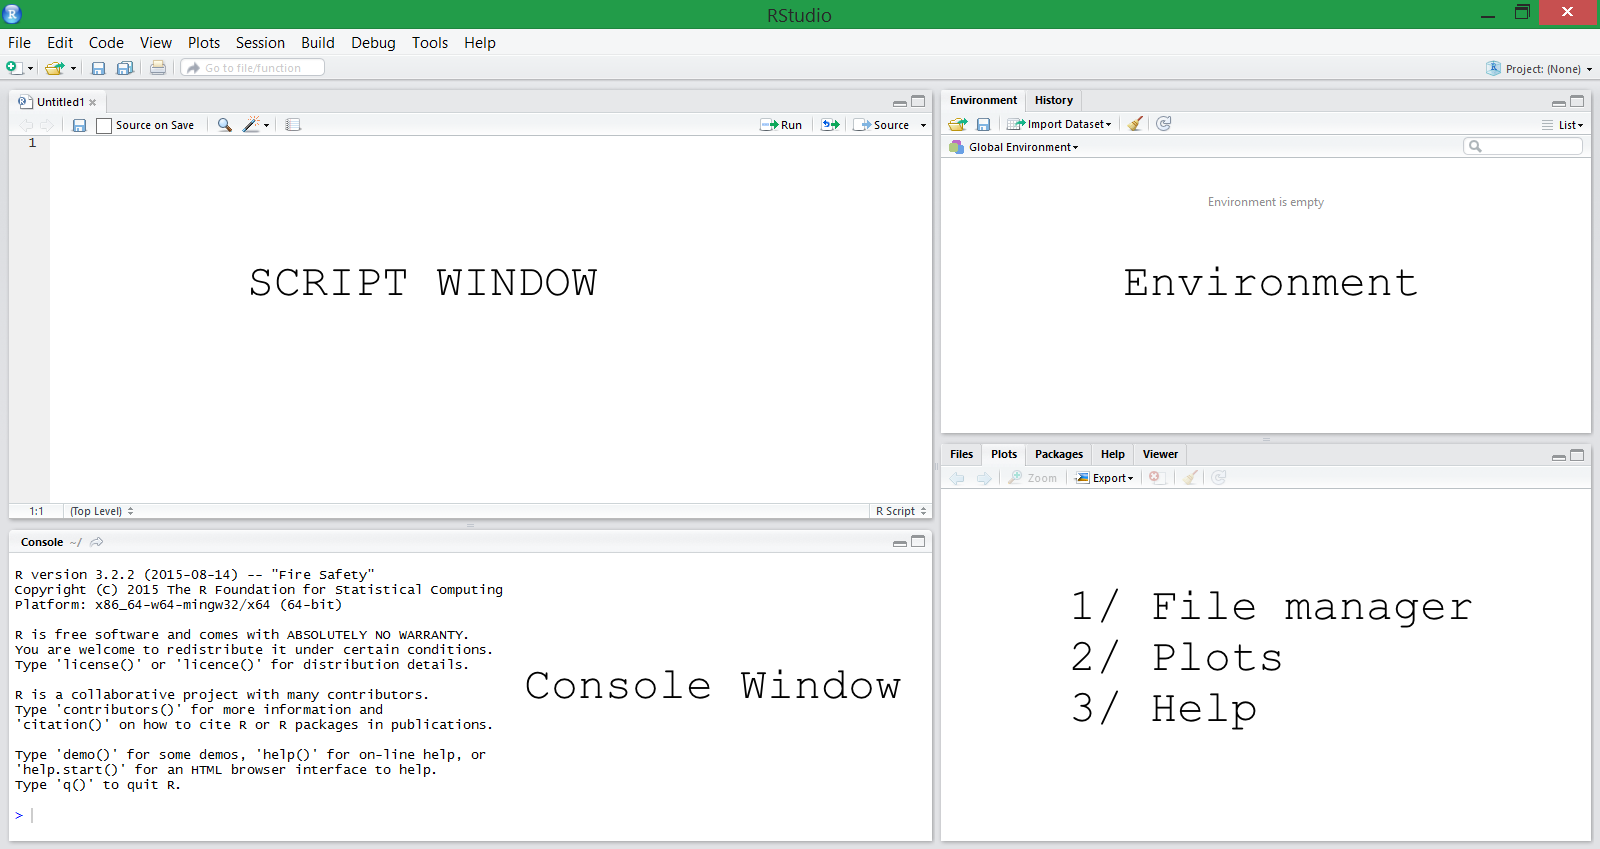
\includegraphics[width=\textwidth]{img/RStudioWindow}
\end{frame}
%%%%%%%%%%%%%%%%%%%%%%%%%%%%%%%%%%%%%%%%%%%%%%%%%%%%%%%%%%%%%%%%%%%%%%%%%%%%%%%%%%%%%%%%%%%%%%%%%%%%


%%%%%%%%%%%%%%%%%%%%%%%%%%%%%%%%%%%%%%%%%%%%%%%%%%%%%%%%%%%%%%%%%%%%%%%%%%%%%%%%%%%%%%%%%%%%%%%%%%%

\begin{frame}{Background}
\begin{itemize}
\item  \RStudio has four panels (we can move and adjust their position in Preferences):
\begin{enumerate}
\item Console panel
\item Source editor
\item Environment panel
\item Files, Plots, and Help panel
\end{enumerate}
\item Let's start by going through these in a little bit more detail.
\end{itemize}
\end{frame}




\begin{frame}[fragile]{RStudio IDE}
\begin{description}
\item[Console] Where commands are executed.  Where you see the input/output.
\item[Script Window] Draft and save code (only input) and run in the console by typing \keystroke{Ctrl}/\keystroke{Cmnd} (Windows/Mac) +\keystroke{Enter}, or pressing  
\includegraphics[height=1.2em]{./img/run.png}.
\item[Environment] Shows saved variables and datasets
\item[File Browser/Plots/Help] Show files in working directory and generated plots, help, open window.
\end{description}
\end{frame}
%%%%%%%



% \begin{frame}{Console panel}
% \begin{itemize}
% \item The console panel is where \R commands are executed.
% \item In this panel you see the \emph{input}/\emph{output}.
% \begin{itemize}
% \item The input can either be typed in real time using the keyboard, or run from a \R \emph{script} (more on this soon)
% \item The output is displayed to the screen.
% \end{itemize}
% \end{itemize}
% \end{frame}


\begin{frame}[fragile]{Console panel}
\begin{itemize}
\item To see how we can use the Console  with keyboard input, simply navigate to the panel and start tying commands:
\begin{knitrout}\footnotesize
\definecolor{shadecolor}{rgb}{0.969, 0.969, 0.969}\color{fgcolor}\begin{kframe}
\begin{alltt}
\hlnum{2}\hlopt{+}\hlnum{4}
\hlkwd{print}\hlstd{(}\hlstr{"Hello World!"}\hlstd{)}
\end{alltt}
\end{kframe}
\end{knitrout}
\item Notice that \R defaults functionality is displays output in the console directely beneith the inputs.
\begin{itemize}
\item Shows {\color{blue} input (blue)}, output (black) and any {\color{red}errors or warnings (red)} (different ``Themes" can be chosen to display different colours).
\end{itemize}
\end{itemize}
\end{frame}


\begin{frame}[fragile]{}
\textbf{Sidenote:} I will be using \href{https://yihui.name/knitr/}{\bf knitr} to produce {\tt R}  lecture notes.  
\begin{itemize}
\item {\tt R} input appears in highlighted text (colour will depend on the object)
\item comments in purple italics, and 
\item output is printed with two preceeding hashtags\footnote[frame]{provides an easy  to copy and paste \R  code}.
% \item The {\tt \#\#} before the output provides an easy way for readers to copy and paste \R source code (since output the output is masked as comments); 
you will not see the two hashtags on standard output in \R and \RStudio.
\end{itemize}
\begin{knitrout}
\definecolor{shadecolor}{rgb}{0.969, 0.969, 0.969}\color{fgcolor}\begin{kframe}
\begin{alltt}
\hlcom{# comments in purple italics}
 \hlnum{2} \hlopt{+} \hlnum{3} \hlcom{# input}
\end{alltt}
\begin{verbatim}
## [1] 5
\end{verbatim}
\begin{alltt}
\hlcom{## ^ denotes output}
\end{alltt}
\end{kframe}
\end{knitrout}
\end{frame}



\begin{frame}[fragile]{R scripts}
\begin{itemize}
\vfill
\item More commonly, we will be executing commands from an \R script.
\vfill
\item An \R \define{script} is a text document containing \R commands and comments (i.e. all of your inputs without any output).
\begin{itemize}
\item Hashtags {\tt \#} indicate the start of a comment.
\item A shortcut to commenting in \RStudio is \keystroke{shift} + \keystroke{Command} + \keystroke{C} on a Mac and \keystroke{shift} + \keystroke{Contrl} + \keystroke{C} on a Windows machine
\end{itemize}
\vfill
\item An R script ends with the extension {\tt .R}
\vfill
\item Apart from one-off calculations, it is always a good idea to save an \R script (e.g. easy to share and reproduce you results)
\vfill
\end{itemize}
\end{frame}


\begin{frame}[fragile]{R scripts}
 A very simple \R script ({\tt script.R} on Canvas):
 \begin{Verbatim}[frame=single,label=script.R, xleftmargin=.5in]
 # Simple addition
 2 + 3 # this is a comment
 # Simple subtraction
 2 - 3
 # Simple multiplication
 print(2*3)
 # Simple power
 2^3 # another comment
 \end{Verbatim}
\end{frame}

\begin{frame}[fragile]{Running R scripts}
\begin{itemize}
\item To run code from an \R script, simply:
\begin{enumerate}
\item open the file (which will have a {\sf .R} extension) in RStudio\footnote[frame]{for the remainder of the course I will assume you are using RStudio}
\item Place your cursor on the line you wish to execute and press 
\includegraphics[width=2.5em]{./img/run.png} or type \keystroke{Cmnd}/\keystroke{Ctrl} (Mac/Windows) + \keystroke{ENTER}
\end{enumerate}
\vfill
\item This will essentially copy and paste the text from the script window into your console window to be run.
\vfill
\item Upon executing a command, your cursor will automatically navigate to the next execuatble command.
\vfill
\end{itemize}
\end{frame}

\begin{frame}[fragile]{Running R scripts}
\begin{itemize}
% \item  To get the output associated with this code we would either step through it line by line (eg using 
\includegraphics[height=1.2em]{./img/run.png}) or source the entire document.
\item \emph{Sourcing} a script is equivalent to running the entire contents of the file in your console.
\vfill
\item To source an R script either:
 \begin{itemize}
 \item Open the .R file in Rstudio and click the 
\includegraphics[height=1.2em]{./img/source.png} button
 \item Open the .R file and type \keystroke{Shift}+\keystroke{Ctrl}+\keystroke{S} (Windows) or \keystroke{Shift}+\keystroke{Cmnd}+\keystroke{S} if you are on a Mac.
 \item Run the following command in your console:
\begin{knitrout}\footnotesize
\definecolor{shadecolor}{rgb}{0.969, 0.969, 0.969}\color{fgcolor}\begin{kframe}
\begin{alltt}
\hlkwd{source}\hlstd{(}\hlstr{"simple.R"}\hlstd{)} \hlcom{# for example}
\end{alltt}
\end{kframe}
\end{knitrout}
\item Note that all lines of code were run, but only the values wraped in {\tt print()} statements appear in the console window.
 \end{itemize}
\end{itemize}
\end{frame}


%%%%%%%%%%%%%%%%%%
\begin{frame}[fragile]{}
The \texttt{print} function will \emph{print} to the standard output (console in RStudio)
\begin{knitrout}\footnotesize
\definecolor{shadecolor}{rgb}{0.969, 0.969, 0.969}\color{fgcolor}\begin{kframe}
\begin{alltt}
\hlkwd{print}\hlstd{(}\hlstr{"Hello World!"}\hlstd{)}
\end{alltt}
\begin{verbatim}
## [1] "Hello World!"
\end{verbatim}
\end{kframe}
\end{knitrout}
Print statements are often used in conjunction with {\tt paste()} functions
\begin{knitrout}\footnotesize
\definecolor{shadecolor}{rgb}{0.969, 0.969, 0.969}\color{fgcolor}\begin{kframe}
\begin{alltt}
\hlstd{x} \hlkwb{=} \hlnum{5}
\hlkwd{print}\hlstd{(}\hlkwd{paste}\hlstd{(}\hlstr{"x ="}\hlstd{, x))}
\end{alltt}
\begin{verbatim}
## [1] "x = 5"
\end{verbatim}
\begin{alltt}
\hlkwd{print}\hlstd{(}\hlkwd{paste}\hlstd{(}\hlstr{"x"}\hlstd{, x,} \hlkwc{sep}\hlstd{=}\hlstr{" = "}\hlstd{))}
\end{alltt}
\begin{verbatim}
## [1] "x = 5"
\end{verbatim}
\begin{alltt}
\hlkwd{print}\hlstd{(}\hlstr{"x="}\hlstd{,x)} \hlcom{# doesn't work like python}
\end{alltt}
\begin{verbatim}
## [1] "x="
\end{verbatim}
\end{kframe}
\end{knitrout}
\end{frame}
%%%%%%%%%%%%%%%%%%%%%%%%%%%%%%%%%%%%%%%%%%%%%%%%%%%%%%%%%%%%%%%%%%%%%%%%%%%%%%%%%%%%%%%%%%%%%%%%%%%%




\begin{frame}[fragile]{Working Directory}
\begin{itemize}
\item Running the \verb|source("simple.R")| command requires that {\tt simple.R} is saved in your current \emph{working directory}.
\vfill
\item The \emph{working directory} is the ``home base'' of your R program. 
\vfill
\item All files are written to and read from the working directory.  
\vfill
\item N.B. If you want to read a file that is not in your working directory, you will have to specify the complete \emph{path}, eg.
\begin{knitrout}\footnotesize
\definecolor{shadecolor}{rgb}{0.969, 0.969, 0.969}\color{fgcolor}\begin{kframe}
\begin{alltt}
\hlcom{# tilde (~) is shortform for your home directory}
\hlkwd{source}\hlstd{(}\hlstr{"~/Dropbox/Data301/08R/data/simple.R"}\hlstd{)}
\end{alltt}
\end{kframe}
\end{knitrout}
\footnotesize{What is my \href{https://en.wikipedia.org/wiki/Home_directory}{home directory}? ({\tt /home/<username>} for Macs)}
\end{itemize}
\end{frame}



\begin{frame}[fragile]{Working Directory}
There are a few ways to set your working directory in RStudio:
\begin{enumerate}
\item Using the \emph{interface} by doing 
\begin{center}
\texttt{Session $\to$ Set Working Directory $\to$ Choose Directory}\\[1em]
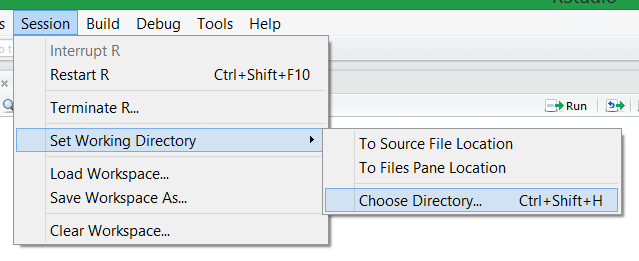
\includegraphics[width=.5\textwidth]{img/session}
\end{center}
\item Using the \texttt{setwd()} command  
\end{enumerate}
\begin{knitrout}\footnotesize
\definecolor{shadecolor}{rgb}{0.969, 0.969, 0.969}\color{fgcolor}\begin{kframe}
\begin{alltt}
\hlkwd{setwd}\hlstd{(}\hlstr{"c:/Documents/my/working/directory"}\hlstd{)}
\end{alltt}
\end{kframe}
\end{knitrout}
N.B. To check your working directory use \texttt{getwd()}.
\end{frame}





% \begin{frame}[fragile]{}
% \begin{itemize}
% \item The \texttt{[1]} in the \R output indicates that the adjacent element is the 1st element printed.
% \item For multiline outputs the number in the square brackets will indicate where the adjacent falls in term of the printed elements.
% \end{itemize}
% \end{frame}
% 
% 
% \begin{frame}[fragile]{}
% <<echo=TRUE, size="small", tidy=FALSE>>=
% longvector = c("this","is","a","long","vector","of",
%     "words","that","will","print","on","multiple","lines")
% longvector
% @
% For example  \texttt{[7]}/\texttt{[13]} indicates that the first element of the second/third line is the 7th/13th element of \texttt{longvector}, repsectively.
% \end{frame}



\begin{frame}[fragile]{Objects and Variables}
\begin{itemize}
\item {\bf Everything} you see or create in \R is an object.
\item This is an abstract term for anything that can be assignment to a varible.
\item A \emph{variable} is a name that refers to a location that stores a data value.
$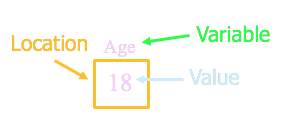
\includegraphics[width=0.5\textwidth]{../../../Data301/Irenes_301_Slides/04VBA/img/Variable.png}$ \\
\begin{alert}
{IMPORTANT:} The \emph{value} at a location can change.% using initialization or assignment.
\end{alert}
\end{itemize}
\end{frame}


% \begin{frame}[fragile]{}
% \begin{itemize}
% \item Notice when you assign something to an object, \R does not automatically print the result to the the screen.
% \item For that reason, when we save output to a variable, we will have to call the varaible name or use a print statment to see our result
% \end{itemize}
% <<>>=
% 2 + 3
% x = 2+3
% x
% # another alternative:
% (x = 2+3)
% @
% \end{frame}


% \section{Data types}
% \begin{frame}[fragile]{Classes}
% \begin{itemize}
% \item There are many \textit{classes} in R and each have different rules.
% \item You can even create your own class in \R (but this is beyond the scope of this course)
% \item The function {\tt class(x)} will tell you what kind of object {\tt x} is.
% \end{itemize}
% \end{frame}



\begin{frame}[fragile]{Some {\tt R} Basics}
\begin{itemize}
\item Like Python, R is case sensitive.\nl
\item Unlike Python, R in not that particular about white space and indent.
\begin{knitrout}\footnotesize
\definecolor{shadecolor}{rgb}{0.969, 0.969, 0.969}\color{fgcolor}\begin{kframe}
\begin{alltt}
      \hlstd{x} \hlkwb{=} \hlnum{5} \hlcom{# both OK!}
\hlstd{x} \hlkwb{=} \hlnum{7}
\end{alltt}
\end{kframe}
\end{knitrout}
\item R commands may be separated either by a semi-colon or a newline (or both).
\begin{knitrout}\footnotesize
\definecolor{shadecolor}{rgb}{0.969, 0.969, 0.969}\color{fgcolor}\begin{kframe}
\begin{alltt}
\hlstd{x} \hlkwb{=} \hlnum{7}
\hlstd{y} \hlkwb{=} \hlnum{3} \hlcom{# or}
\hlstd{x} \hlkwb{=} \hlnum{7}\hlstd{; y} \hlkwb{=} \hlnum{3}
\hlstd{x} \hlkwb{=} \hlnum{7}\hlstd{;} \hlcom{# ok too}
\end{alltt}
\end{kframe}
\end{knitrout}
\end{itemize}
\end{frame}


\begin{frame}[fragile]{Basics of R}
\vfill
 We can either use the {\tt =} or {\tt <-} for the assignment operator.  There is some debate on the \href{https://csgillespie.wordpress.com/2010/11/16/assignment-operators-in-r-vs/}{preferred syntax}
\begin{knitrout}\footnotesize
\definecolor{shadecolor}{rgb}{0.969, 0.969, 0.969}\color{fgcolor}\begin{kframe}
\begin{alltt}
\hlstd{x} \hlkwb{<-} \hlnum{5}\hlstd{;} \hlcom{# both OK!}
\hlstd{x} \hlkwb{=} \hlnum{5}
\end{alltt}
\end{kframe}
\end{knitrout}
Curly brackets $\{$ $\}$ are used to group commands together.
\begin{knitrout}\footnotesize
\definecolor{shadecolor}{rgb}{0.969, 0.969, 0.969}\color{fgcolor}\begin{kframe}
\begin{alltt}
\hlkwa{for} \hlstd{(i} \hlkwa{in} \hlkwd{c}\hlstd{(}\hlnum{1}\hlstd{,}\hlnum{2}\hlstd{,}\hlnum{3}\hlstd{)) \{}
  \hlkwd{print}\hlstd{(i)}
  \hlkwd{print}\hlstd{(i} \hlopt{+} \hlnum{1}\hlstd{)}
\hlkwd{print}\hlstd{(i} \hlopt{-} \hlnum{1}\hlstd{)}  \hlcom{# indent doesn't matter}
\hlstd{\}}
\end{alltt}
\end{kframe}
\end{knitrout}
\end{frame}



\begin{frame}[fragile]{Basic Operations for Vectors}\label{basic}
We can also perform basic operations on vectors:
\begin{center}
\begin{tabular}{ll}
Operation & Command \\\hline 
natural log & \verb!log(x)!\\
Exponent & \verb!exp(x)!\\
Log base 10 & \verb!log10(x)!\\
Absolute value & \verb!abs(x)!\\
Square root & \verb!sqrt(x)!\\
Sum & \verb!sum(x)!\\
Number of elements in $x$  & \verb!length(x)!\\
\end{tabular}
\end{center}
\end{frame}


\begin{frame}[fragile]{}
\begin{center}
\begin{tabular}{ll}
Unique elements of $x$ & \verb!unique(x)!\\
Mean & \verb!mean(x)!\\
Variance & \verb!var(x)!\\
Standard Deviation & \verb!sd(x)!\\
Minimum value & \verb!min(x)!\\
Maximum value & \verb!max(x)!\\
Smallest and largest values  & \verb!range(x)!\\
median & \verb!median(x)!\\
Basic statistical summary & \verb!summary(x)!\\
Sort & \verb!sort(x)!\\
\end{tabular}
\end{center}
\end{frame}





%%%%%%%%%%%%%%%%%%%%%%%%%%%%%%%%%%%%%%%%%%%%%%%%%%%%%%%%%%%%%%%%%%%%%%%%%%%%%%%%%%%%%%%%%%%%%%%%%%%%
\begin{frame}[fragile]
\begin{question}
How many of the following are true?
\begin{enumerate}
\item R is case-sensitive.
\item A command in R can be terminated by a semi-colon. 
\item Indentation is the syntax used to group statements together. 
\item A single line comment starts with \#. 
\end{enumerate}
\begin{multicols}{5}
\begin{enumerate}[A)]
\item 0
\item 1
\item 2
\item 3
\item 4
\end{enumerate}
\end{multicols}
\end{question}
\end{frame}


\begin{frame}<handout:0>[fragile]
\begin{question}
How many of the following are true?
\begin{enumerate}
\item R is case-sensitive. \onslide<+->\pcmark
\item A command in R can be terminated by a semi-colon. \pcmark
\item Indentation is the syntax used to group statements together. \pxmark
\item A single line comment starts with \#. \pcmark
\end{enumerate}
\begin{multicols}{5}
\begin{enumerate}[A)]
\item 0
\item 1
\item 2
\item \tans{6}{3}
\item 4
\end{enumerate}
\end{multicols}
\end{question}
\end{frame}


%%%%%%%%%%%%%%%%%%%%%%%%%%%%%%%%%%%
% Question ########################
%%%%%%%%%%%%%%%%%%%%%%%%%%%%%%%%%%%



\begin{frame}[fragile]
\begin{question}
 How many of the are following statements are true?
  \begin{itemize}
 \item {In RStudio, R commands are executed in the console window} %T
 \item {R scripts store both R input and output} %F
 \item {We can run R without RStudio but we cannotrun Rstudio without R} %T
 \item {A working directory can not be changed once an R session is started} %F
\end{itemize}
\end{question}
\begin{multicols}{5}
\begin{enumerate}[A)]
\item 0
\item 1
\item 2
\item 3
\item 4
\end{enumerate}
\end{multicols}
\end{frame}


 %%%%%%%%%%%%%%%%%%%%%%%%%%%%%%%%%%%
 % Answer ########################
 %%%%%%%%%%%%%%%%%%%%%%%%%%%%%%%%%%%
 
\begin{frame}<handout:0>[fragile]
\begin{question}
 How many of the are following statements are true?
  \begin{itemize}
 \item {In RStudio, R commands are executed in the console window} %T
 \onslide<+->{}\pcmark
 \item {R scripts store both R input and output} %F
 \pxmark
 \item {We can run R without RStudio but we cannotrun Rstudio without R} %T
 \pcmark
 \item {A working directory can not be changed once an R session is started} %F
 \pxmark
\end{itemize}
\end{question}
\begin{multicols}{5}
\begin{enumerate}[A)]
\item 0
\item 1
\item \tans{5}{2}
\item 3
\item 4
\end{enumerate}
\end{multicols}
\end{frame}




\begin{frame}[fragile]{Data types}
\begin{itemize}
\item Here's a list of some important data types used in R:
 \begin{enumerate}
\item Integer (Whole Numbers)
\item Numeric (Real Numbers)
\item Character
\item Logical (Boolean TRUE/FALSE)
\item Factor 
\item Complex (we won't focus on this type)
 \end{enumerate}
 \item As with Python, variables of certain types need not be declared, and {\tt R} will do its best at determining the most appropriate data type.
 \item We can check the type of an object using {\tt class()}
 %\footnote[frame]{We could also use {\tt typeof()}, see the \href{https://stat.ethz.ch/R-manual/R-devel/doc/manual/R-lang.html#Objects}{R Language Definition} manual, and more about their differences \href{http://rfunction.com/archives/770}{here}}
\end{itemize}
\end{frame}



\begin{frame}[fragile]{}
\begin{knitrout}\footnotesize
\definecolor{shadecolor}{rgb}{0.969, 0.969, 0.969}\color{fgcolor}\begin{kframe}
\begin{alltt}
\hlcom{# class works like type() in Python}
\hlkwd{class}\hlstd{(}\hlnum{1}\hlstd{)}   \hlcom{# like Python float type}
\end{alltt}
\begin{verbatim}
## [1] "numeric"
\end{verbatim}
\begin{alltt}
\hlkwd{class}\hlstd{(}\hlkwd{as.integer}\hlstd{(}\hlnum{1}\hlstd{))} \hlcom{# like Python int type}
\end{alltt}
\begin{verbatim}
## [1] "integer"
\end{verbatim}
\begin{alltt}
\hlstd{z} \hlkwb{=} \hlnum{1} \hlopt{+} \hlnum{2i}\hlstd{;} \hlkwd{class}\hlstd{(z)}
\end{alltt}
\begin{verbatim}
## [1] "complex"
\end{verbatim}
\begin{alltt}
\hlkwd{class}\hlstd{(}\hlnum{TRUE}\hlstd{)} \hlcom{# notice all in caps!  (True in Python)}
\end{alltt}
\begin{verbatim}
## [1] "logical"
\end{verbatim}
\begin{alltt}
\hlkwd{class}\hlstd{(}\hlstr{"irene"}\hlstd{)} \hlcom{# like Python string}
\end{alltt}
\begin{verbatim}
## [1] "character"
\end{verbatim}
\end{kframe}
\end{knitrout}
\end{frame}



\begin{frame}[fragile]{Numeric and Integer}
\begin{itemize}
\item Often the default storage of numbers in \R is in as numeric.
\vfill
\item To force a variable to be an interger, we need to use the {\tt as.integer()} function, or use the  ``L'' suffix.
\end{itemize}
\begin{knitrout}\footnotesize
\definecolor{shadecolor}{rgb}{0.969, 0.969, 0.969}\color{fgcolor}\begin{kframe}
\begin{alltt}
\hlstd{numobj} \hlkwb{=} \hlnum{2} \hlcom{# numeric (not integer)}
\hlkwd{as.integer}\hlstd{(numobj)} \hlcom{# integer}
\end{alltt}
\begin{verbatim}
## [1] 2
\end{verbatim}
\begin{alltt}
\hlstd{intobj} \hlkwb{=} \hlnum{2L} \hlcom{# integer }
\hlkwd{as.integer}\hlstd{(}\hlstr{'4'}\hlstd{)} \hlcom{# like int() in Python}
\end{alltt}
\begin{verbatim}
## [1] 4
\end{verbatim}
\end{kframe}
\end{knitrout}
{\footnotesize N.B. forcing data to be a certain type is called \href{https://bookdown.org/rdpeng/rprogdatascience/r-nuts-and-bolts.html\#explicit-coercion}{data coercion}. See slide \ref{coercion}}
\end{frame}

\begin{frame}[fragile]{Character}
\begin{itemize}
\item A single letter or string of characters will be recorded as a {\tt character} object. 
\item  You can use double quotes or single quotes for all of these specifications (just be consistent)
\begin{knitrout}\footnotesize
\definecolor{shadecolor}{rgb}{0.969, 0.969, 0.969}\color{fgcolor}\begin{kframe}
\begin{alltt}
\hlcom{# note our usage of quotes }
\hlstd{charobj} \hlkwb{=} \hlstr{"s"}
\hlstd{strobj} \hlkwb{=} \hlstr{'string'}
\hlstd{numstr} \hlkwb{=} \hlkwd{as.character}\hlstd{(}\hlnum{4}\hlstd{)} \hlcom{# like str(4) in Python}
\hlcom{# badobj = "str' # unmatched quotes = bad}
\end{alltt}
\end{kframe}
\end{knitrout}
\end{itemize}
\end{frame}

\begin{frame}[fragile]{Aside}{Auto-complete}
Notice that \R trys to help us out by autocompleting our quotes (i.e. when we type one quotation/parenthesis the closing one will appear automatically.  If you don't like this feature, you can turn it off (but I suggest you keep it!)
\end{frame}



\begin{frame}[fragile]{Logical}
In \R, \texttt{T} and \texttt{F} are reserved for logicals (i.e. True/False objects) and \R reads \texttt{T} the same as \texttt{TRUE} or \texttt{F} the same as \texttt{FALSE}. %Inside of
\begin{knitrout}\footnotesize
\definecolor{shadecolor}{rgb}{0.969, 0.969, 0.969}\color{fgcolor}\begin{kframe}
\begin{alltt}
\hlstd{x} \hlkwb{=} \hlkwd{c}\hlstd{(T,} \hlnum{FALSE}\hlstd{,}\hlnum{TRUE}\hlstd{, F)} \hlcom{# notice we don't use quotes}
\hlstd{x}
\end{alltt}
\begin{verbatim}
## [1]  TRUE FALSE  TRUE FALSE
\end{verbatim}
\end{kframe}
\end{knitrout}
 Oftentimes, True and False conditions are coded as 0 and 1s.  To covert them to logical, use {\tt as.logical()}. %Similar functions are available for the other data types; namely, {\tt as.numeric}.
\begin{knitrout}\footnotesize
\definecolor{shadecolor}{rgb}{0.969, 0.969, 0.969}\color{fgcolor}\begin{kframe}
\begin{alltt}
\hlkwd{as.logical}\hlstd{(}\hlnum{0}\hlstd{)}
\end{alltt}
\begin{verbatim}
## [1] FALSE
\end{verbatim}
\begin{alltt}
\hlkwd{as.logical}\hlstd{(}\hlnum{1}\hlstd{)}
\end{alltt}
\begin{verbatim}
## [1] TRUE
\end{verbatim}
\end{kframe}
\end{knitrout}
\end{frame}


\begin{frame}[fragile]{Factor}
\begin{itemize}
\item If you want a variable to be a factor type (so that different symbols are regarded as a level), use \texttt{var=factor(var)}.
\begin{knitrout}\footnotesize
\definecolor{shadecolor}{rgb}{0.969, 0.969, 0.969}\color{fgcolor}\begin{kframe}
\begin{alltt}
\hlstd{notfactor} \hlkwb{=} \hlkwd{c}\hlstd{(}\hlstr{"H"}\hlstd{,}\hlstr{"M"}\hlstd{,} \hlstr{"M"}\hlstd{,} \hlstr{"L"}\hlstd{,} \hlstr{"H"}\hlstd{)}
\hlstd{notfactor}
\end{alltt}
\begin{verbatim}
## [1] "H" "M" "M" "L" "H"
\end{verbatim}
\begin{alltt}
\hlstd{(fvec} \hlkwb{=} \hlkwd{factor}\hlstd{(notfactor))}
\end{alltt}
\begin{verbatim}
## [1] H M M L H
## Levels: H L M
\end{verbatim}
\begin{alltt}
\hlkwd{levels}\hlstd{(fvec)} \hlcom{# to see the levels}
\end{alltt}
\begin{verbatim}
## [1] "H" "L" "M"
\end{verbatim}
\end{kframe}
\end{knitrout}
\end{itemize}
\end{frame}

% factor(x, levels=c(100, 200, 400, 500), ordered=TRUE) Add this
% https://www.r-exercises.com/2015/12/28/factor-exercises/


%% If z <- factor(c("p", "q", "p", "r", "q")) and levels of z are "p", "q" ,"r", write an R expression that will change the level "p" to "w" so that z is equal to: "w", "q" , "w", "r" , "q".
% z <- factor(c("p", "q", "p", "r", "q"))
% levels(z)[1] <- "w"

%Let x <- data.frame(q=c(2, 4, 6), p=c("a", "b", "c")). Write an R statement that will replace levels a, b, c with labels "fertiliser1", "fertliser2", "fertiliser3".
% x <- data.frame(q=c(2, 4, 6), p=c("a", "b", "c"))
% x$p <- factor(x$p, levels=c("a", "b", "c"), labels=c("fertiliser1", "fertiliser2", "fertiliser3"))


\begin{frame}[fragile]{Factor}
\begin{itemize}
\item 
We also have the option to specify the labels to something more meaningful:
\begin{knitrout}\footnotesize
\definecolor{shadecolor}{rgb}{0.969, 0.969, 0.969}\color{fgcolor}\begin{kframe}
\begin{alltt}
\hlcom{# make sure your labels appear in the same order as levels(fvec) }
\hlstd{fvec} \hlkwb{=} \hlkwd{factor}\hlstd{(}\hlkwc{x}\hlstd{=notfactor,} \hlkwc{labels}\hlstd{=}\hlkwd{c}\hlstd{(}\hlstr{"High"}\hlstd{,}\hlstr{"Low"}\hlstd{,}\hlstr{"Medium"}\hlstd{))}
\hlstd{fvec}
\end{alltt}
\begin{verbatim}
## [1] High   Medium Medium Low    High  
## Levels: High Low Medium
\end{verbatim}
\end{kframe}
\end{knitrout}
\end{itemize}
\end{frame}


\begin{frame}[fragile]{Ordered Factors}
Sometimes the order of the factors do not matter (eg. eye colour).  If however we want to specify some meaningful order, we could use levels.  In this example, since {\tt L} (low) $<$ {\tt M} (medium) $<$ {\tt H} (high), we could specify ordered levels using {\tt ordered = TRUE}:
\begin{knitrout}\footnotesize
\definecolor{shadecolor}{rgb}{0.969, 0.969, 0.969}\color{fgcolor}\begin{kframe}
\begin{alltt}
\hlstd{(fvec} \hlkwb{=} \hlkwd{factor}\hlstd{(}\hlkwc{x}\hlstd{=notfactor,} \hlkwc{levels}\hlstd{=}\hlkwd{c}\hlstd{(}\hlstr{"L"}\hlstd{,}\hlstr{"M"}\hlstd{,}\hlstr{"H"}\hlstd{)))}
\end{alltt}
\begin{verbatim}
## [1] H M M L H
## Levels: L M H
\end{verbatim}
\begin{alltt}
\hlstd{(fvec2} \hlkwb{=} \hlkwd{factor}\hlstd{(}\hlkwc{x}\hlstd{=notfactor,} \hlkwc{levels}\hlstd{=}\hlkwd{c}\hlstd{(}\hlstr{"L"}\hlstd{,}\hlstr{"M"}\hlstd{,}\hlstr{"H"}\hlstd{),} \hlkwc{ordered} \hlstd{=} \hlnum{TRUE}\hlstd{))}
\end{alltt}
\begin{verbatim}
## [1] H M M L H
## Levels: L < M < H
\end{verbatim}
\end{kframe}
\end{knitrout}
\end{frame}


\begin{frame}[fragile]{Ordered Factors}
Notice how we can compare the levels in {\tt fvec2} using relational operators whereas in {\tt fvec} we cannot:
\begin{knitrout}\footnotesize
\definecolor{shadecolor}{rgb}{0.969, 0.969, 0.969}\color{fgcolor}\begin{kframe}
\begin{alltt}
\hlstd{fvec[}\hlnum{1}\hlstd{]}\hlopt{>}\hlstd{fvec[}\hlnum{3}\hlstd{]}
\end{alltt}


{\ttfamily\noindent\color{warningcolor}{\#\# Warning in Ops.factor(fvec[1], fvec[3]): '>' not meaningful for factors}}\begin{verbatim}
## [1] NA
\end{verbatim}
\begin{alltt}
\hlstd{fvec2[}\hlnum{1}\hlstd{]}\hlopt{>}\hlstd{fvec2[}\hlnum{3}\hlstd{]}
\end{alltt}
\begin{verbatim}
## [1] TRUE
\end{verbatim}
\begin{alltt}
\hlkwd{print}\hlstd{(}\hlkwd{paste}\hlstd{(fvec2[}\hlnum{1}\hlstd{],} \hlstr{"is treated as greater than"}\hlstd{, fvec[}\hlnum{3}\hlstd{]))}
\end{alltt}
\begin{verbatim}
## [1] "H is treated as greater than M"
\end{verbatim}
\end{kframe}
\end{knitrout}
\end{frame}



\begin{frame}[fragile]{Ordered Factors}
We could use this in conjunction with {\tt labels}:
\begin{knitrout}\footnotesize
\definecolor{shadecolor}{rgb}{0.969, 0.969, 0.969}\color{fgcolor}\begin{kframe}
\begin{alltt}
\hlstd{fvec3} \hlkwb{=} \hlkwd{factor}\hlstd{(}\hlkwc{x}\hlstd{=notfactor,} \hlkwc{levels}\hlstd{=}\hlkwd{c}\hlstd{(}\hlstr{"L"}\hlstd{,}\hlstr{"M"}\hlstd{,}\hlstr{"H"}\hlstd{),} \hlkwc{labels}\hlstd{=}\hlkwd{c}\hlstd{(}\hlstr{"Low"}\hlstd{,}\hlstr{"Medium"}\hlstd{,} \hlstr{"High"}\hlstd{),} \hlkwc{ordered} \hlstd{=}\hlnum{TRUE}\hlstd{)}
\hlstd{fvec3}
\end{alltt}
\begin{verbatim}
## [1] High   Medium Medium Low    High  
## Levels: Low < Medium < High
\end{verbatim}
\end{kframe}
\end{knitrout}
\end{frame}


% \begin{frame}[fragile]{Aside}{Notation}
% \begin{itemize}
% \item We say that {\tt factor()} is a \define{function} for which we have specified two \define{arguments} (having argument names: {\tt from}, {\tt x} and {\tt labels}).
% \item You can access the help file to see the details of this function using {\tt ?factor}
% \item Notice that is has other (optional) arguments that we haven't specified.  
% \end{itemize}
% \end{frame}


\begin{frame}[fragile]{Factor}
\begin{itemize}
\item The case my also arise that we need to specify levels not seen in the data set.  In that case we can specify the {\tt levels} argument:
\item Using {\tt letters} a built in vector containing the 26 letters of the alphabet;
\begin{knitrout}\footnotesize
\definecolor{shadecolor}{rgb}{0.969, 0.969, 0.969}\color{fgcolor}\begin{kframe}
\begin{alltt}
\hlstd{x} \hlkwb{=} \hlkwd{c}\hlstd{(}\hlstr{"o"}\hlstd{,}\hlstr{"q"}\hlstd{,}\hlstr{"h"}\hlstd{,}\hlstr{"n"}\hlstd{,}\hlstr{"s"}\hlstd{,}\hlstr{"b"}\hlstd{,}\hlstr{"u"}\hlstd{,}\hlstr{"d"}\hlstd{,}\hlstr{"p"}\hlstd{,}\hlstr{"r"}\hlstd{)}
\hlstd{xlist} \hlkwb{=} \hlkwd{factor}\hlstd{(x,} \hlkwc{levels}\hlstd{=letters)}
\hlkwd{table}\hlstd{(xlist)}
\end{alltt}
\begin{verbatim}
## xlist
## a b c d e f g h i j k l m n o p q r s t u v w x y z 
## 0 1 0 1 0 0 0 1 0 0 0 0 0 1 1 1 1 1 1 0 1 0 0 0 0 0
\end{verbatim}
\end{kframe}
\end{knitrout}
\end{itemize}
\end{frame}


\begin{frame}[fragile]{Aside}{Built-in Constants}
\begin{itemize}
\item On the previous slide we used the built-in constant {\tt letters}
\item Other build in constants include:
\begin{itemize}
\item {\tt LETTERS} (capital letters)
\item {\tt month.name} (eg. ``January", ``February", etc..)
\item {\tt month.abb} (eg. ``Jan", ``Feb", etc..)
\item {\tt pi} 3.141593
\end{itemize}
\end{itemize}
\end{frame}


\begin{frame}[fragile]{Try it: in R}
\begin{question}
In an R program
\begin{enumerate}
\item Make a comment with your name and student number.
\item Calculate the following $4 \times 5 - 12^3$, ${\rm e}^{3 \times 4}$, $\sin(4\pi-6)$.
\item Guess then check with \texttt{class} the types of the following variables
\begin{knitrout}\footnotesize
\definecolor{shadecolor}{rgb}{0.969, 0.969, 0.969}\color{fgcolor}\begin{kframe}
\begin{alltt}
\hlstd{var1} \hlkwb{<-} \hlnum{FALSE}
\hlstd{var2} \hlkwb{<-} \hlstd{T}
\hlstd{var3} \hlkwb{<-} \hlstr{"TRUE"}
\hlstd{var4} \hlkwb{<-} \hlnum{3}\hlopt{^}\hlnum{4} \hlopt{-} \hlnum{10}
\hlstd{var5} \hlkwb{<-} \hlstr{"Hello World!"}
\end{alltt}
\end{kframe}
\end{knitrout}
\end{enumerate}
\end{question}
\end{frame}
%%%%%%%%%%%%%%%%%%%%%%%%%%%%%%%%%%%%%%%%%%%%%%%%%%%%%%%%%%%%%%%%%%%%%%%%%%%%%%%%%%




\begin{frame}[fragile]{Data structures}
\begin{itemize}
\item R has a wide variety of data structures including:
\begin{itemize}
\item scalars, eg
\begin{knitrout}\footnotesize
\definecolor{shadecolor}{rgb}{0.969, 0.969, 0.969}\color{fgcolor}\begin{kframe}
\begin{alltt}
\hlstd{scalar1} \hlkwb{<-} \hlnum{1}
\hlstd{scalar2} \hlkwb{<-} \hlstr{"string"}
\end{alltt}
\end{kframe}
\end{knitrout}
\item vectors (numerical, character, logical)
\begin{knitrout}\footnotesize
\definecolor{shadecolor}{rgb}{0.969, 0.969, 0.969}\color{fgcolor}\begin{kframe}
\begin{alltt}
\hlstd{vec1} \hlkwb{<-} \hlkwd{c}\hlstd{(}\hlnum{1}\hlstd{,}\hlnum{2}\hlstd{,}\hlnum{3}\hlstd{); vec2} \hlkwb{<-} \hlkwd{c}\hlstd{(}\hlstr{"one"}\hlstd{,} \hlstr{"two"}\hlstd{,} \hlstr{"three"}\hlstd{)}
\hlstd{vec3} \hlkwb{<-} \hlkwd{c}\hlstd{(}\hlnum{TRUE}\hlstd{,} \hlnum{FALSE}\hlstd{, T)}
\end{alltt}
\end{kframe}
\end{knitrout}

\item matrices
\item data frames, and
\item lists
\end{itemize}
\end{itemize}
\end{frame}



\begin{frame}[fragile]{Vectors}
\begin{itemize}
\item A vector is the most basic data structure in \R and can be of two types:
\begin{itemize}
\item atomic vectors
\item lists
\end{itemize}
\item As we did in the examples above, you can create a vector using \texttt{c} (see {\tt ?c}\footnote[frame]{you can get help on any function running {\tt ?functionname}} for more details on this \textit{combine} function)
\end{itemize}
\end{frame}


\begin{frame}[fragile]{Vectors}
Atomic Vectors can be \emph{either} vectors characters, logical, integers or numeric (but can \emph{not} mix types)
\begin{knitrout}\footnotesize
\definecolor{shadecolor}{rgb}{0.969, 0.969, 0.969}\color{fgcolor}\begin{kframe}
\begin{alltt}
\hlcom{# example of a numeric vector:}
\hlstd{y}\hlkwb{=}\hlkwd{c}\hlstd{(}\hlnum{2}\hlstd{,}\hlnum{3}\hlstd{,}\hlnum{0}\hlstd{,}\hlnum{3}\hlstd{,}\hlnum{1}\hlstd{,}\hlnum{0}\hlstd{,}\hlnum{0}\hlstd{,}\hlnum{1}\hlstd{)}
\hlcom{# example of a character vector:}
\hlstd{letters}\hlkwb{<-}\hlkwd{c}\hlstd{(}\hlstr{'A'}\hlstd{,}\hlstr{'B'}\hlstd{,}\hlstr{'C'}\hlstd{)}
\hlcom{# example of a logical vector:}
\hlstd{lvec} \hlkwb{<-} \hlkwd{c}\hlstd{(}\hlnum{TRUE}\hlstd{,} \hlnum{FALSE}\hlstd{,} \hlnum{FALSE}\hlstd{)}
\end{alltt}
\end{kframe}
\end{knitrout}
Unlike Python lists, we cannot mix types within vectors:
\begin{knitrout}\footnotesize
\definecolor{shadecolor}{rgb}{0.969, 0.969, 0.969}\color{fgcolor}\begin{kframe}
\begin{alltt}
\hlcom{# the integer 1 gets converted to character}
\hlkwd{print}\hlstd{(vec} \hlkwb{<-} \hlkwd{c}\hlstd{(}\hlnum{1}\hlstd{,} \hlstr{"a"}\hlstd{,} \hlstr{"b"}\hlstd{))}
\end{alltt}
\begin{verbatim}
## [1] "1" "a" "b"
\end{verbatim}
\end{kframe}
\end{knitrout}
\end{frame}



\begin{frame}[fragile]{coercion}\label{coercion}
\begin{itemize}
\item By \textit{atomic vectors} we mean they can only take on one data type. 
\item If we specify more than one type in a single vector, \R will  convert the mixed types to a single type which it deems most appropriate.
\item The \emph{coercion} will move towards the one that's easiest to coerce to.
\item You can coerce vectors explicitly using the {\tt as.<}\textit{type}{\tt>} (eg. {\tt as.numeric}, {\tt as.character}, etc. )
\end{itemize}
\end{frame}

\begin{frame}[fragile]{}
\begin{knitrout}\footnotesize
\definecolor{shadecolor}{rgb}{0.969, 0.969, 0.969}\color{fgcolor}\begin{kframe}
\begin{alltt}
\hlstd{(x} \hlkwb{=} \hlkwd{c}\hlstd{(}\hlstr{"apple"}\hlstd{,} \hlnum{2}\hlstd{,} \hlnum{TRUE}\hlstd{))} \hlcom{# converts all to character}
\end{alltt}
\begin{verbatim}
## [1] "apple" "2"     "TRUE"
\end{verbatim}
\begin{alltt}
\hlstd{(x} \hlkwb{=} \hlkwd{c}\hlstd{(}\hlnum{TRUE}\hlstd{,} \hlnum{4}\hlstd{))} \hlcom{# converts all to numeric}
\end{alltt}
\begin{verbatim}
## [1] 1 4
\end{verbatim}
\begin{alltt}
\hlstd{(x} \hlkwb{=} \hlkwd{c}\hlstd{(}\hlnum{2L}\hlstd{,} \hlopt{-}\hlnum{1.3}\hlstd{))} \hlcom{# converts to numeric}
\end{alltt}
\begin{verbatim}
## [1]  2.0 -1.3
\end{verbatim}
\begin{alltt}
\hlstd{(x} \hlkwb{=} \hlkwd{c}\hlstd{(}\hlnum{TRUE}\hlstd{,} \hlnum{0}\hlstd{,} \hlnum{1}\hlstd{,} \hlnum{FALSE}\hlstd{))} \hlcom{# converts all to numeric}
\end{alltt}
\begin{verbatim}
## [1] 1 0 1 0
\end{verbatim}
\begin{alltt}
\hlkwd{as.logical}\hlstd{(}\hlkwc{x} \hlstd{=} \hlkwd{c}\hlstd{(}\hlnum{TRUE}\hlstd{,} \hlnum{0}\hlstd{,} \hlnum{1}\hlstd{,} \hlnum{FALSE}\hlstd{))} \hlcom{# converts to logical}
\end{alltt}
\begin{verbatim}
## [1]  TRUE FALSE  TRUE FALSE
\end{verbatim}
\end{kframe}
\end{knitrout}
\end{frame}



\begin{frame}[fragile]{Vectors}
Numeric vectors can be created a number of different ways. 
\begin{knitrout}\footnotesize
\definecolor{shadecolor}{rgb}{0.969, 0.969, 0.969}\color{fgcolor}\begin{kframe}
\begin{alltt}
\hlcom{# Ceate a vector of size 10, where each element is a 2:}
\hlstd{y} \hlkwb{=} \hlkwd{rep}\hlstd{(}\hlnum{2}\hlstd{,}\hlnum{10}\hlstd{)}
\hlcom{# This specifies a sequence of integers:}
\hlstd{y} \hlkwb{=} \hlnum{3}\hlopt{:}\hlnum{12}
\hlcom{#This specifies a sequence of real numbers:}
\hlstd{z} \hlkwb{=} \hlkwd{seq}\hlstd{(}\hlkwc{from}\hlstd{=}\hlnum{3}\hlstd{,}\hlkwc{to}\hlstd{=}\hlnum{12}\hlstd{,}\hlkwc{by}\hlstd{=}\hlnum{1}\hlstd{)} \hlcom{# by = 1 is the default}
\hlcom{#This specifies a sequence of real numbers:}
\hlstd{z} \hlkwb{=} \hlkwd{seq}\hlstd{(}\hlkwc{from}\hlstd{=}\hlnum{2}\hlstd{,}\hlkwc{to}\hlstd{=}\hlnum{1}\hlstd{,}\hlkwc{by}\hlstd{=}\hlopt{-}\hlnum{0.1}\hlstd{)}
\end{alltt}
\end{kframe}
\end{knitrout}
\begin{alertblock}{The {\tt end} in {\tt seq()} \emph{is} inclusive}
{\tt seq()} is like the Python {\tt range(start, end, step)} function, only now, {\tt end} \textit{\bf is} inclusive!
\end{alertblock}
\end{frame}


\begin{frame}[fragile]{Aside}{Notation}
\begin{itemize}
\item We say that {\tt seq()} is a \define{function} for which we have specified three \define{arguments} (having argument names: {\tt from}, {\tt to} and {\tt by}).
\item Assuming we are putting the values in the correct order, you do not need to specify the argument names explicitly.
\begin{knitrout}\footnotesize
\definecolor{shadecolor}{rgb}{0.969, 0.969, 0.969}\color{fgcolor}\begin{kframe}
\begin{alltt}
\hlkwd{seq}\hlstd{(}\hlnum{1}\hlstd{,}\hlnum{2}\hlstd{,}\hlnum{0.1}\hlstd{)} \hlcom{# same as seq(from=1,to=2,by=0.1)}
\end{alltt}
\begin{verbatim}
##  [1] 1.0 1.1 1.2 1.3 1.4 1.5 1.6 1.7 1.8 1.9 2.0
\end{verbatim}
\begin{alltt}
\hlcom{# if we want to specify arguments out of order, }
\hlcom{# we HAVE to include argument names:}
\hlkwd{seq}\hlstd{(}\hlkwc{by}\hlstd{=}\hlnum{0.1}\hlstd{,} \hlkwc{to}\hlstd{=}\hlnum{2}\hlstd{,} \hlkwc{from}\hlstd{=}\hlnum{1}\hlstd{)} \hlcom{# arguments in green}
\end{alltt}
\begin{verbatim}
##  [1] 1.0 1.1 1.2 1.3 1.4 1.5 1.6 1.7 1.8 1.9 2.0
\end{verbatim}
\end{kframe}
\end{knitrout}
\end{itemize}
\end{frame}




\begin{frame}[fragile,label={seed}]{Vectors}
Here are some ways you can generate \emph{``random"} data in {\tt R}:

\begin{knitrout}\footnotesize
\definecolor{shadecolor}{rgb}{0.969, 0.969, 0.969}\color{fgcolor}\begin{kframe}
\begin{alltt}
\hlcom{# Ceates a vector of size 10, of random numbers between 0 and 1}
\hlstd{y} \hlkwb{=} \hlkwd{runif}\hlstd{(}\hlnum{10}\hlstd{)}
\hlcom{# Creates a vector of size 3 sampled from x without replacement}
\hlstd{(y} \hlkwb{=} \hlkwd{sample}\hlstd{(}\hlkwc{x}\hlstd{=}\hlkwd{c}\hlstd{(}\hlnum{1}\hlstd{,}\hlnum{2}\hlstd{,}\hlnum{3}\hlstd{),} \hlkwc{size}\hlstd{=}\hlnum{3}\hlstd{))}
\end{alltt}
\begin{verbatim}
## [1] 1 3 2
\end{verbatim}
\begin{alltt}
\hlstd{(y} \hlkwb{=} \hlkwd{sample}\hlstd{(}\hlkwc{x}\hlstd{=}\hlkwd{c}\hlstd{(}\hlnum{1}\hlstd{,}\hlnum{2}\hlstd{,}\hlnum{3}\hlstd{),} \hlkwc{size}\hlstd{=}\hlnum{3}\hlstd{))} \hlcom{# random output each time}
\end{alltt}
\begin{verbatim}
## [1] 3 2 1
\end{verbatim}
\begin{alltt}
\hlcom{# Creates a vector of size 3 sampled from x with replacement}
\hlstd{(y} \hlkwb{=} \hlkwd{sample}\hlstd{(}\hlkwc{x}\hlstd{=}\hlkwd{c}\hlstd{(}\hlnum{1}\hlstd{,}\hlnum{2}\hlstd{,}\hlnum{3}\hlstd{),} \hlkwc{size}\hlstd{=}\hlnum{3}\hlstd{,} \hlkwc{replace}\hlstd{=}\hlnum{TRUE}\hlstd{))}
\end{alltt}
\begin{verbatim}
## [1] 3 2 3
\end{verbatim}
\end{kframe}
\end{knitrout}

\end{frame}

\begin{frame}[fragile]{Vectors}
We can also create empty vectors
\begin{knitrout}\footnotesize
\definecolor{shadecolor}{rgb}{0.969, 0.969, 0.969}\color{fgcolor}\begin{kframe}
\begin{alltt}
\hlstd{x} \hlkwb{<-} \hlkwd{vector}\hlstd{()} \hlcom{# defaults to logical (FALSE)}
\hlstd{x} \hlkwb{<-} \hlkwd{vector}\hlstd{(}\hlkwc{length} \hlstd{=} \hlnum{10}\hlstd{)} \hlcom{# defaults to logical vec of FALSES}
\hlstd{x} \hlkwb{<-} \hlkwd{vector}\hlstd{(}\hlstr{"character"}\hlstd{,} \hlkwc{length} \hlstd{=} \hlnum{10}\hlstd{)}
\hlstd{x} \hlkwb{<-} \hlkwd{vector}\hlstd{(}\hlstr{"numeric"}\hlstd{,}   \hlkwc{length} \hlstd{=} \hlnum{10}\hlstd{)}
\hlstd{x} \hlkwb{<-} \hlkwd{vector}\hlstd{(}\hlstr{"integer"}\hlstd{,}   \hlkwc{length} \hlstd{=} \hlnum{10}\hlstd{)}
\hlstd{x} \hlkwb{<-} \hlkwd{vector}\hlstd{(}\hlstr{"logical"}\hlstd{,}   \hlkwc{length} \hlstd{=} \hlnum{10}\hlstd{)}
\end{alltt}
\end{kframe}
\end{knitrout}
Notice the difference in creating empty vectors in R from Python.  For instance, the following will produce an error
\begin{knitrout}\footnotesize
\definecolor{shadecolor}{rgb}{0.969, 0.969, 0.969}\color{fgcolor}\begin{kframe}
\begin{alltt}
x <- ()
\end{alltt}


{\ttfamily\noindent\bfseries\color{errorcolor}{\#\# Error: <text>:1:7: unexpected ')'\\\#\# 1: x <- ()\\\#\#\ \ \ \ \ \ \ \ \ \  \textasciicircum{}}}\end{kframe}
\end{knitrout}

\end{frame}

% 
% \begin{frame}[fragile]{Seed}
% \begin{itemize}
% \item Notice that I use {\tt set.seed(4758)} on \hyperlink{seed}{\beamerbutton{slide}} \ref{seed}.
% \item This was created so that when you run the same exact code on our computer, you will obtain the same `random' numbers.
% \item A random seed is a number used to initialize a pseudorandom number generator.
% \item Without going into to much detail, setting a seed using {\tt set.seed} will yield same `random` results every time.
% \end{itemize}
% \end{frame}
% 
% 
% \begin{frame}[fragile]{}
% <<>>=
% set.seed(4444)
% runif(1)
% set.seed(4444)
% runif(1)
% runif(1)
% @
% \end{frame}


\begin{frame}[fragile]{Scalars}
Scalars are just vectors of length 1.  To check the length of any vector use {\tt length()}
\begin{knitrout}\footnotesize
\definecolor{shadecolor}{rgb}{0.969, 0.969, 0.969}\color{fgcolor}\begin{kframe}
\begin{alltt}
\hlstd{x} \hlkwb{=} \hlnum{4}\hlstd{;} \hlkwd{length}\hlstd{(x)}
\end{alltt}
\begin{verbatim}
## [1] 1
\end{verbatim}
\begin{alltt}
\hlstd{y}\hlkwb{=}\hlkwd{c}\hlstd{(}\hlnum{2}\hlstd{,}\hlnum{3}\hlstd{,}\hlnum{0}\hlstd{,}\hlnum{3}\hlstd{,}\hlnum{1}\hlstd{,}\hlnum{0}\hlstd{,}\hlnum{0}\hlstd{,}\hlnum{1}\hlstd{);} \hlkwd{length}\hlstd{(y)}
\end{alltt}
\begin{verbatim}
## [1] 8
\end{verbatim}
\begin{alltt}
\hlcom{# notice that this does not count characters in a string:}
\hlkwd{length}\hlstd{(}\hlstr{"Hello"}\hlstd{)} \hlcom{# see nchar("Hello") for # of characters}
\end{alltt}
\begin{verbatim}
## [1] 1
\end{verbatim}
\end{kframe}
\end{knitrout}
\begin{alertblock}{{\tt length()} in {\tt R} instead of {\tt len()} in Python}
{\tt length} solely provides the length of a vector/list.
\end{alertblock}
\end{frame}

\begin{frame}[fragile]{Indexing Vectors}
To index an element from a vector, use single square brackets
\begin{knitrout}\footnotesize
\definecolor{shadecolor}{rgb}{0.969, 0.969, 0.969}\color{fgcolor}\begin{kframe}
\begin{alltt}
\hlstd{z} \hlkwb{=} \hlkwd{c}\hlstd{(}\hlstr{"apples"}\hlstd{,}\hlstr{"bananas"}\hlstd{,}\hlstr{"oranges"}\hlstd{,} \hlstr{"pineapples"}\hlstd{); z[}\hlnum{1}\hlstd{]}
\end{alltt}
\begin{verbatim}
## [1] "apples"
\end{verbatim}
\begin{alltt}
\hlstd{z[}\hlnum{2}\hlopt{:}\hlnum{3}\hlstd{]}
\end{alltt}
\begin{verbatim}
## [1] "bananas" "oranges"
\end{verbatim}
\begin{alltt}
\hlstd{z[}\hlkwd{c}\hlstd{(}\hlnum{4}\hlstd{,}\hlnum{2}\hlstd{)]}
\end{alltt}
\begin{verbatim}
## [1] "pineapples" "bananas"
\end{verbatim}
\begin{alltt}
\hlstd{z[}\hlopt{-}\hlnum{1}\hlstd{]} \hlcom{# removes the first item in the vector}
\end{alltt}
\begin{verbatim}
## [1] "bananas"    "oranges"    "pineapples"
\end{verbatim}
\end{kframe}
\end{knitrout}
\begin{alertblock}{Notice that the index begins at 1 NOT 0!!!!!!}
Also notice the difference in the \verb|[-1]| notation.
\end{alertblock}

\end{frame}


\begin{frame}[fragile]{}
We have the option of including names for our vector elements (similar to a Python dictionary)
\begin{knitrout}\footnotesize
\definecolor{shadecolor}{rgb}{0.969, 0.969, 0.969}\color{fgcolor}\begin{kframe}
\begin{alltt}
\hlstd{z} \hlkwb{=} \hlkwd{c}\hlstd{(}\hlnum{123456}\hlstd{,} \hlnum{25}\hlstd{,} \hlnum{2019}\hlstd{);} \hlkwd{names}\hlstd{(z)} \hlkwb{<-} \hlkwd{c}\hlstd{(}\hlstr{"studentID"}\hlstd{,}\hlstr{"age"}\hlstd{,}\hlstr{"year"}\hlstd{)}
\hlstd{z[}\hlstr{"studentID"}\hlstd{]} \hlcom{# same as z[1]}
\end{alltt}
\begin{verbatim}
## studentID 
##    123456
\end{verbatim}
\begin{alltt}
\hlstd{z[}\hlkwd{c}\hlstd{(}\hlstr{"age, year"}\hlstd{)]} \hlcom{# wont work like z[c(2,3)]}
\end{alltt}
\begin{verbatim}
## <NA> 
##   NA
\end{verbatim}
\begin{alltt}
\hlstd{z[}\hlkwd{c}\hlstd{(}\hlnum{FALSE}\hlstd{,} \hlnum{TRUE}\hlstd{,} \hlnum{TRUE}\hlstd{)]} \hlcom{# index using logicals (same as z[c(1,2)]) }
\end{alltt}
\begin{verbatim}
##  age year 
##   25 2019
\end{verbatim}
\begin{alltt}
\hlstd{z[}\hlopt{-}\hlstr{"year"}\hlstd{]} \hlcom{# wont work like z[-3]}
\end{alltt}


{\ttfamily\noindent\bfseries\color{errorcolor}{\#\# Error in -"{}year"{}: invalid argument to unary operator}}\end{kframe}
\end{knitrout}
\end{frame}

\begin{frame}[fragile]{}
To add a new element/delete/replace an element:
\begin{knitrout}\footnotesize
\definecolor{shadecolor}{rgb}{0.969, 0.969, 0.969}\color{fgcolor}\begin{kframe}
\begin{alltt}
\hlstd{z} \hlkwb{=} \hlkwd{c}\hlstd{(}\hlstr{"first"}\hlstd{,}\hlstr{"second"}\hlstd{,}\hlstr{"third"}\hlstd{,} \hlstr{"fourth"}\hlstd{)}
\hlcom{# adds a fith element and replaces the second}
\hlstd{z[}\hlnum{5}\hlstd{]} \hlkwb{=} \hlstr{"fifth"}\hlstd{;  z[}\hlnum{2}\hlstd{]} \hlkwb{=} \hlstr{"2nd"}
\hlstd{z}
\end{alltt}
\begin{verbatim}
## [1] "first"  "2nd"    "third"  "fourth" "fifth"
\end{verbatim}
\begin{alltt}
\hlcom{#removes the second element}
\hlstd{(z} \hlkwb{=} \hlstd{z[}\hlopt{-}\hlnum{2}\hlstd{])}
\end{alltt}
\begin{verbatim}
## [1] "first"  "third"  "fourth" "fifth"
\end{verbatim}
\end{kframe}
\end{knitrout}
R does not use methods like the {\tt .append()} as Python did. %Also note how we can assign a new element using square brackets and the a
\end{frame}

\begin{frame}[fragile]{}
Notice what happens if we add a 10th element to z (without specifying elements 6--9):
\begin{knitrout}\footnotesize
\definecolor{shadecolor}{rgb}{0.969, 0.969, 0.969}\color{fgcolor}\begin{kframe}
\begin{alltt}
\hlstd{z[}\hlnum{10}\hlstd{]} \hlkwb{=} \hlstr{"tenth"}
\hlstd{z}
\end{alltt}
\begin{verbatim}
##  [1] "first"  "third"  "fourth" "fifth"  NA       NA       NA      
##  [8] NA       NA       "tenth"
\end{verbatim}
\end{kframe}
\end{knitrout}
\end{frame}

\begin{frame}[fragile]{}
We can also add new named elements
\begin{knitrout}\footnotesize
\definecolor{shadecolor}{rgb}{0.969, 0.969, 0.969}\color{fgcolor}\begin{kframe}
\begin{alltt}
\hlstd{z} \hlkwb{=} \hlkwd{c}\hlstd{(}\hlnum{123456}\hlstd{,} \hlnum{25}\hlstd{,} \hlnum{2019}\hlstd{);} \hlkwd{names}\hlstd{(z)} \hlkwb{<-} \hlkwd{c}\hlstd{(}\hlstr{"studentID"}\hlstd{,}\hlstr{"age"}\hlstd{,}\hlstr{"year"}\hlstd{)}
\hlcom{# adds a forth element with the students major}
\hlstd{z[}\hlstr{"major"}\hlstd{]} \hlkwb{=} \hlstr{"COSC"}
\hlstd{z}
\end{alltt}
\begin{verbatim}
## studentID       age      year     major 
##  "123456"      "25"    "2019"    "COSC"
\end{verbatim}
\end{kframe}
\end{knitrout}
Notice how the addition of this forth element cuase the vector to change to a vector of characters (because of data \hyperlink{coercion}{coercion}!)
\end{frame}

\begin{frame}[fragile]{Vector Operations}

\begin{itemize}
\item Basic operations (like the ones outlined on slide \ref{basic}) can be a applied to vectors.
\vfill
\item Like the {\tt map} function and numpy arrays in Python, these functions will be applied \textit{elementwise}.
\end{itemize}
\begin{knitrout}\footnotesize
\definecolor{shadecolor}{rgb}{0.969, 0.969, 0.969}\color{fgcolor}\begin{kframe}
\begin{alltt}
\hlstd{(y}\hlkwb{=} \hlkwd{sample}\hlstd{(}\hlnum{1}\hlopt{:}\hlnum{20}\hlstd{,} \hlnum{9}\hlstd{))} \hlcom{# samples 9 random numbers from 1 to 20}
\end{alltt}
\begin{verbatim}
## [1] 15 19 14  3 10  2  6 11  5
\end{verbatim}
\begin{alltt}
\hlnum{2} \hlopt{*} \hlstd{y} \hlcom{# multiplies each element by 2}
\end{alltt}
\begin{verbatim}
## [1] 30 38 28  6 20  4 12 22 10
\end{verbatim}
\begin{alltt}
\hlstd{y} \hlopt{+} \hlstd{y} \hlcom{# equivalent}
\end{alltt}
\begin{verbatim}
## [1] 30 38 28  6 20  4 12 22 10
\end{verbatim}
\end{kframe}
\end{knitrout}
\end{frame}


\begin{frame}[fragile]{Vector Operations}
\begin{itemize}
\item Notice that operations like {\tt sort()} do not change the input vector unless that vector is reassigned.
\end{itemize}
\begin{knitrout}\footnotesize
\definecolor{shadecolor}{rgb}{0.969, 0.969, 0.969}\color{fgcolor}\begin{kframe}
\begin{alltt}
\hlkwd{print}\hlstd{(y)}
\end{alltt}
\begin{verbatim}
## [1] 15 19 14  3 10  2  6 11  5
\end{verbatim}
\begin{alltt}
\hlkwd{sort}\hlstd{(y)}
\end{alltt}
\begin{verbatim}
## [1]  2  3  5  6 10 11 14 15 19
\end{verbatim}
\begin{alltt}
\hlkwd{print}\hlstd{(y)}
\end{alltt}
\begin{verbatim}
## [1] 15 19 14  3 10  2  6 11  5
\end{verbatim}
\begin{alltt}
\hlcom{# this time reassign it}
\hlstd{y} \hlkwb{=} \hlkwd{sort}\hlstd{(y,} \hlkwc{decreasing} \hlstd{=} \hlnum{TRUE}\hlstd{)}
\hlkwd{print}\hlstd{(y)}
\end{alltt}
\begin{verbatim}
## [1] 19 15 14 11 10  6  5  3  2
\end{verbatim}
\end{kframe}
\end{knitrout}
% summary(y)
\end{frame}


\begin{frame}[fragile]{Matrices}
\begin{itemize}
\item \define{Matrices} can be viewed as column vectors stacked side by side or row vectors stack one on top of another
\vfill
\item In \R, matrices are really just a multi-dimensional vector (similar to numpy \emph{arrays} in Python)
\vfill
\item The main difference between matrices and the vectors discussed in the previous slides is that a matrix has a \define{dimension} (similar the \emph{shape} of an numpy array in Python). 
\vfill
\item The dimenions can be found using the {\tt dim()} function. 
\end{itemize}
\end{frame}


\begin{frame}[fragile]{Matrices}
\begin{knitrout}\footnotesize
\definecolor{shadecolor}{rgb}{0.969, 0.969, 0.969}\color{fgcolor}\begin{kframe}
\begin{alltt}
\hlstd{(m} \hlkwb{<-} \hlkwd{matrix}\hlstd{(}\hlnum{1}\hlopt{:}\hlnum{8}\hlstd{,} \hlkwc{nrow} \hlstd{=} \hlnum{2}\hlstd{,} \hlkwc{ncol} \hlstd{=} \hlnum{4}\hlstd{))}
\end{alltt}
\begin{verbatim}
##      [,1] [,2] [,3] [,4]
## [1,]    1    3    5    7
## [2,]    2    4    6    8
\end{verbatim}
\begin{alltt}
\hlkwd{dim}\hlstd{(m)} \hlcom{# gives the number or rows and columns}
\end{alltt}
\begin{verbatim}
## [1] 2 4
\end{verbatim}
\begin{alltt}
\hlkwd{class}\hlstd{(m)}
\end{alltt}
\begin{verbatim}
## [1] "matrix"
\end{verbatim}
\end{kframe}
\end{knitrout}
\end{frame}

\begin{frame}[fragile]{Matrices}
\begin{itemize}
\item By default, matrices are constructed columnwise.  
\item You can always change to row-wise by specifying {\tt byrow=TRUE}
\end{itemize}
\begin{knitrout}\footnotesize
\definecolor{shadecolor}{rgb}{0.969, 0.969, 0.969}\color{fgcolor}\begin{kframe}
\begin{alltt}
\hlstd{(m} \hlkwb{<-} \hlkwd{matrix}\hlstd{(}\hlnum{1}\hlopt{:}\hlnum{6}\hlstd{,} \hlkwc{nrow}\hlstd{=}\hlnum{2}\hlstd{,} \hlkwc{ncol} \hlstd{=}\hlnum{3}\hlstd{))} \hlcom{# fill columnwise}
\end{alltt}
\begin{verbatim}
##      [,1] [,2] [,3]
## [1,]    1    3    5
## [2,]    2    4    6
\end{verbatim}
\begin{alltt}
\hlstd{(m} \hlkwb{<-} \hlkwd{matrix}\hlstd{(}\hlnum{1}\hlopt{:}\hlnum{6}\hlstd{,} \hlkwc{nrow}\hlstd{=}\hlnum{2}\hlstd{,} \hlkwc{ncol} \hlstd{=}\hlnum{3}\hlstd{,} \hlkwc{byrow}\hlstd{=}\hlnum{TRUE}\hlstd{))} \hlcom{#fill row-wise}
\end{alltt}
\begin{verbatim}
##      [,1] [,2] [,3]
## [1,]    1    2    3
## [2,]    4    5    6
\end{verbatim}
\end{kframe}
\end{knitrout}
\end{frame}


\begin{frame}[fragile]{Matrices}
An alternative way of constructing matrices is to use {\tt array()}
\begin{knitrout}\footnotesize
\definecolor{shadecolor}{rgb}{0.969, 0.969, 0.969}\color{fgcolor}\begin{kframe}
\begin{alltt}
\hlkwd{array}\hlstd{(}\hlnum{1}\hlopt{:}\hlnum{6}\hlstd{,} \hlkwc{dim}\hlstd{=}\hlkwd{c}\hlstd{(}\hlnum{2}\hlstd{,}\hlnum{3}\hlstd{))} \hlcom{# a 2 x 3 array  (2 dimensional)}
\end{alltt}
\begin{verbatim}
##      [,1] [,2] [,3]
## [1,]    1    3    5
## [2,]    2    4    6
\end{verbatim}
\begin{alltt}
\hlcom{# returns 2 matrices of dimension 4 x 3}
\hlstd{(arr3d} \hlkwb{<-}  \hlkwd{array}\hlstd{(}\hlnum{1}\hlopt{:}\hlnum{24}\hlstd{,} \hlkwc{dim}\hlstd{=}\hlkwd{c}\hlstd{(}\hlnum{4}\hlstd{,}\hlnum{3}\hlstd{,}\hlnum{2}\hlstd{)))} \hlcom{# a 4 x 3 x 2 array (3 dimensional)}
\end{alltt}
\begin{verbatim}
## , , 1
## 
##      [,1] [,2] [,3]
## [1,]    1    5    9
## [2,]    2    6   10
## [3,]    3    7   11
## [4,]    4    8   12
## 
## , , 2
## 
##      [,1] [,2] [,3]
## [1,]   13   17   21
## [2,]   14   18   22
## [3,]   15   19   23
## [4,]   16   20   24
\end{verbatim}
\end{kframe}
\end{knitrout}
\end{frame}


\begin{frame}[fragile]{Array visualization}
  Image adapted from \href{https://www.slideshare.net/smitparikh1/multidimensional-array/3}{(image source)}
\begin{center}
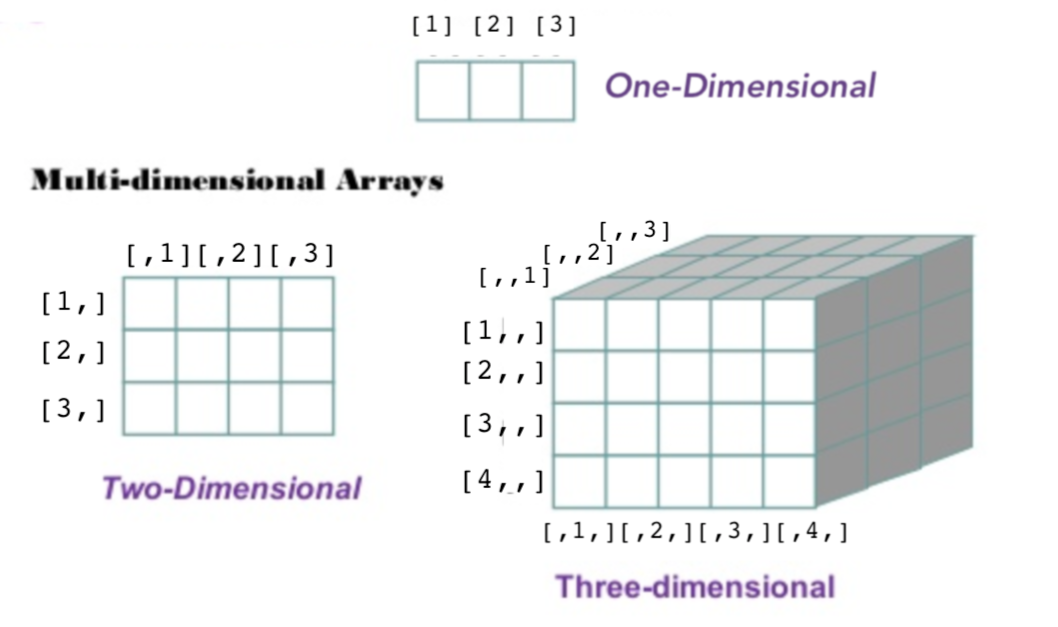
\includegraphics[height=0.72\textheight, width=0.8\textwidth]{img/arrays}
\end{center}
\end{frame}




\begin{frame}[fragile]{Named Matrices}
We may also choose to name our rows and columns
\begin{knitrout}\footnotesize
\definecolor{shadecolor}{rgb}{0.969, 0.969, 0.969}\color{fgcolor}\begin{kframe}
\begin{alltt}
\hlkwd{rownames}\hlstd{(m)} \hlkwb{=} \hlkwd{c}\hlstd{(}\hlstr{"row1"}\hlstd{,} \hlstr{"row2"}\hlstd{)}
\hlkwd{colnames}\hlstd{(m)} \hlkwb{=} \hlkwd{c}\hlstd{(}\hlstr{"col1"}\hlstd{,} \hlstr{"col2"}\hlstd{,} \hlstr{"col3"}\hlstd{)}
\hlstd{m}
\end{alltt}
\begin{verbatim}
##      col1 col2 col3
## row1    1    2    3
## row2    4    5    6
\end{verbatim}
\end{kframe}
\end{knitrout}
\end{frame}


\begin{frame}[fragile]{Indexing}
\begin{itemize}
\item To index an element from a matrix, we can again use square brackets, but we need to specify TWO numbers {\tt[row, col]}.
\vfill
\item To index an element from a higher dimensional array, we use square brackets with as many indeces as there are dimensions {\tt[row, col, dept]} for 3-dimensional arrays.
\vfill
\item  If we want to extract an entire row, we'll leave the {\tt col} field blank (indicating we want all colums).
\vfill
\item  If we want to extract an entire column, we'll leave the {\tt row} field blank (indicating we want all rows).
\vfill
\end{itemize}
\end{frame}

\begin{frame}[fragile]{Indexing}
The following extracts a column, row, and cell from matrix {\tt m},
\begin{knitrout}\footnotesize
\definecolor{shadecolor}{rgb}{0.969, 0.969, 0.969}\color{fgcolor}\begin{kframe}
\begin{alltt}
\hlstd{m[,}\hlnum{3}\hlstd{]} \hlcom{# extract the third column of m}
\end{alltt}
\begin{verbatim}
## row1 row2 
##    3    6
\end{verbatim}
\begin{alltt}
\hlstd{m[}\hlnum{1}\hlstd{,]} \hlcom{# extract the first row of m}
\end{alltt}
\begin{verbatim}
## col1 col2 col3 
##    1    2    3
\end{verbatim}
\begin{alltt}
\hlstd{m[}\hlnum{1}\hlstd{,}\hlnum{3}\hlstd{]} \hlcom{# extract the element in the 1st row and 3rd column}
\end{alltt}
\begin{verbatim}
## [1] 3
\end{verbatim}
\begin{alltt}
\hlstd{arr3d[}\hlnum{4}\hlstd{,}\hlnum{3}\hlstd{,}\hlnum{2}\hlstd{]} \hlcom{# 4th row and 3rd column from the 2nd matrix}
\end{alltt}
\begin{verbatim}
## [1] 24
\end{verbatim}
\end{kframe}
\end{knitrout}
\end{frame}

\begin{frame}[fragile]{}
Alternatively we could call them by name
\begin{knitrout}\footnotesize
\definecolor{shadecolor}{rgb}{0.969, 0.969, 0.969}\color{fgcolor}\begin{kframe}
\begin{alltt}
\hlcom{# extract the third column of m}
\hlstd{m[,}\hlstr{"col3"}\hlstd{]} \hlcom{# same as m[,3]}
\end{alltt}
\begin{verbatim}
## row1 row2 
##    3    6
\end{verbatim}
\begin{alltt}
\hlcom{# extract the first row of m}
\hlstd{m[}\hlstr{"row1"}\hlstd{,]} \hlcom{# same as m[1,]}
\end{alltt}
\begin{verbatim}
## col1 col2 col3 
##    1    2    3
\end{verbatim}
\begin{alltt}
\hlcom{# extract the element in the 1st row and 3rd column}
\hlstd{m[}\hlstr{"row1"}\hlstd{,}\hlstr{"col3"}\hlstd{]} \hlcom{# same as m[1,3]}
\end{alltt}
\begin{verbatim}
## [1] 3
\end{verbatim}
\end{kframe}
\end{knitrout}
\end{frame}


\begin{frame}[fragile]{Indexing}
Note that we can also use one number (tricker this way)
\begin{knitrout}\footnotesize
\definecolor{shadecolor}{rgb}{0.969, 0.969, 0.969}\color{fgcolor}\begin{kframe}
\begin{alltt}
\hlstd{(m} \hlkwb{=} \hlkwd{matrix}\hlstd{(}\hlnum{11}\hlopt{:}\hlnum{4}\hlstd{,} \hlnum{2}\hlstd{,}\hlnum{4}\hlstd{))}
\end{alltt}
\begin{verbatim}
##      [,1] [,2] [,3] [,4]
## [1,]   11    9    7    5
## [2,]   10    8    6    4
\end{verbatim}
\begin{alltt}
\hlstd{m[}\hlnum{8}\hlstd{]} \hlcom{# extracts the 8th element in m}
\end{alltt}
\begin{verbatim}
## [1] 4
\end{verbatim}
\begin{alltt}
\hlstd{(mVector} \hlkwb{=} \hlkwd{as.numeric}\hlstd{(m))}
\end{alltt}
\begin{verbatim}
## [1] 11 10  9  8  7  6  5  4
\end{verbatim}
\begin{alltt}
\hlstd{mVector[}\hlnum{8}\hlstd{]}
\end{alltt}
\begin{verbatim}
## [1] 4
\end{verbatim}
\end{kframe}
\end{knitrout}
\end{frame}

\begin{frame}[fragile]{Indexing}
Like the vectors discussed earlier, matices fall under the atomic vector category and therefore can only store data of one type:
\begin{knitrout}\footnotesize
\definecolor{shadecolor}{rgb}{0.969, 0.969, 0.969}\color{fgcolor}\begin{kframe}
\begin{alltt}
\hlstd{m} \hlkwb{=} \hlkwd{matrix}\hlstd{(}\hlkwd{c}\hlstd{(}\hlstr{"bananas"}\hlstd{,} \hlnum{2}\hlstd{,} \hlnum{TRUE}\hlstd{,} \hlnum{0}\hlstd{),}  \hlkwc{nrow}\hlstd{=}\hlnum{2}\hlstd{,} \hlkwc{ncol}\hlstd{=}\hlnum{2}\hlstd{)}
\hlcom{# notice how all coerce to characters:}
\hlstd{m}
\end{alltt}
\begin{verbatim}
##      [,1]      [,2]  
## [1,] "bananas" "TRUE"
## [2,] "2"       "0"
\end{verbatim}
\end{kframe}
\end{knitrout}
\end{frame}




\begin{frame}[fragile]{lists}
\begin{itemize}
\item
If we want our vector to contain objects of different data types we need to create a list.
\vfill
\item We can think of lists as a special type of vector that can mix data types and  structures
\begin{itemize}
\item For example, an element in a list can contain yet another list (i.e nested lists)
\end{itemize}
\vfill
\item These are very similar to Python lists but remember R lists start with the index 1 and Python lists start with the index 0.
\vfill
\end{itemize}
\end{frame}

\begin{frame}[fragile]{}
 Notice how lists do not force all elements to be of the same type (as was the case with atomic vectors)
\begin{knitrout}\scriptsize
\definecolor{shadecolor}{rgb}{0.969, 0.969, 0.969}\color{fgcolor}\begin{kframe}
\begin{alltt}
\hlstd{(x} \hlkwb{=} \hlkwd{list}\hlstd{(}\hlstr{"apple"}\hlstd{,} \hlnum{2}\hlstd{,} \hlnum{TRUE}\hlstd{))}
\end{alltt}
\begin{verbatim}
## [[1]]
## [1] "apple"
## 
## [[2]]
## [1] 2
## 
## [[3]]
## [1] TRUE
\end{verbatim}
\begin{alltt}
\hlstd{(y} \hlkwb{=} \hlkwd{c}\hlstd{(}\hlstr{"apple"}\hlstd{,}\hlnum{2}\hlstd{,}\hlnum{TRUE}\hlstd{))}
\end{alltt}
\begin{verbatim}
## [1] "apple" "2"     "TRUE"
\end{verbatim}
\end{kframe}
\end{knitrout}

\end{frame}


\begin{frame}[fragile]{lists}
Unlike vectors, the member of a list are accessed using double square brackets:
\begin{knitrout}\footnotesize
\definecolor{shadecolor}{rgb}{0.969, 0.969, 0.969}\color{fgcolor}\begin{kframe}
\begin{alltt}
\hlstd{x[[}\hlnum{1}\hlstd{]]} \hlcom{# first member}
\end{alltt}
\begin{verbatim}
## [1] "apple"
\end{verbatim}
\begin{alltt}
\hlstd{x[[}\hlnum{2}\hlstd{]]} \hlcom{# second member, and so on ...}
\end{alltt}
\begin{verbatim}
## [1] 2
\end{verbatim}
\end{kframe}
\end{knitrout}
\end{frame}

\begin{frame}[fragile]{lists}{(my) notation}
\begin{itemize}
\item While I have specified each member to be a single word/number/logical, we could also have specified them to be vectors or matrices or another list! 
\vfill
\item In an attempt to avoid confusion, I will use \emph{\it member}s to refer to the elements of the \underline{list} and \emph{\it elements} to refer to elements within the \underline{vectors}/\underline{matrices}.
\vfill
\end{itemize}
\end{frame}

\begin{frame}[fragile]{lists}{Indexing}
\begin{itemize}
\item Members will be referenced using double square brackets \verb|[[]]|
\vfill
\item We will reference the elements within each member using square brackets:
\begin{itemize}
\item single square brackets if its a vector \verb|[]|
\item double square brackets if its a list \verb|[[]]|
\end{itemize}
\vfill
\item Notice how R outputs uses the same square bracket referencing in the standard output.
\end{itemize}
\end{frame}


\begin{frame}[fragile]{}
\begin{knitrout}\footnotesize
\definecolor{shadecolor}{rgb}{0.969, 0.969, 0.969}\color{fgcolor}\begin{kframe}
\begin{alltt}
\hlstd{(y} \hlkwb{=} \hlkwd{list}\hlstd{(}\hlkwd{c}\hlstd{(}\hlstr{"apples"}\hlstd{,} \hlstr{"banana"}\hlstd{,} \hlstr{"four"}\hlstd{),} \hlkwd{list}\hlstd{(}\hlnum{1}\hlopt{:}\hlnum{3}\hlstd{,}\hlstr{"hi"}\hlstd{),} \hlkwd{matrix}\hlstd{(}\hlnum{1}\hlopt{:}\hlnum{6}\hlstd{,}\hlnum{2}\hlstd{)))}
\end{alltt}
\begin{verbatim}
## [[1]]
## [1] "apples" "banana" "four"  
## 
## [[2]]
## [[2]][[1]]
## [1] 1 2 3
## 
## [[2]][[2]]
## [1] "hi"
## 
## 
## [[3]]
##      [,1] [,2] [,3]
## [1,]    1    3    5
## [2,]    2    4    6
\end{verbatim}
\begin{alltt}
\hlstd{y[[}\hlnum{3}\hlstd{]][}\hlnum{2}\hlstd{,}\hlnum{3}\hlstd{]}
\end{alltt}
\begin{verbatim}
## [1] 6
\end{verbatim}
\end{kframe}
\end{knitrout}
\end{frame}

\begin{frame}[fragile]{}
The first memeber of {\tt y} is a vector.  We therefore reference its elements by a single index in square brackets
\begin{knitrout}\footnotesize
\definecolor{shadecolor}{rgb}{0.969, 0.969, 0.969}\color{fgcolor}\begin{kframe}
\begin{alltt}
\hlstd{y[[}\hlnum{1}\hlstd{]]} \hlcom{# this is a vector}
\end{alltt}
\begin{verbatim}
## [1] "apples" "banana" "four"
\end{verbatim}
\begin{alltt}
\hlcom{# the third element of this vector is obtained in the usual way}
\hlstd{y[[}\hlnum{1}\hlstd{]][}\hlnum{3}\hlstd{]}
\end{alltt}
\begin{verbatim}
## [1] "four"
\end{verbatim}
\end{kframe}
\end{knitrout}
If it helps, you can think of \verb|y[[1]]| as a new vector object.
\begin{knitrout}\footnotesize
\definecolor{shadecolor}{rgb}{0.969, 0.969, 0.969}\color{fgcolor}\begin{kframe}
\begin{alltt}
\hlstd{(new} \hlkwb{=} \hlstd{y[[}\hlnum{1}\hlstd{]])} \hlcom{# this is a vector}
\end{alltt}
\begin{verbatim}
## [1] "apples" "banana" "four"
\end{verbatim}
\begin{alltt}
\hlstd{new[}\hlnum{1}\hlstd{]}
\end{alltt}
\begin{verbatim}
## [1] "apples"
\end{verbatim}
\end{kframe}
\end{knitrout}
\end{frame}

\begin{frame}[fragile]{}
The second memeber of {\tt y} is \textit{another} list.  We therefore reference its elements by double square brackets
\begin{knitrout}\footnotesize
\definecolor{shadecolor}{rgb}{0.969, 0.969, 0.969}\color{fgcolor}\begin{kframe}
\begin{alltt}
\hlstd{y[[}\hlnum{2}\hlstd{]]}
\end{alltt}
\begin{verbatim}
## [[1]]
## [1] 1 2 3
## 
## [[2]]
## [1] "hi"
\end{verbatim}
\end{kframe}
\end{knitrout}
If it helps, you can think of \verb|y[[2]]| as a new list object
\begin{knitrout}\footnotesize
\definecolor{shadecolor}{rgb}{0.969, 0.969, 0.969}\color{fgcolor}\begin{kframe}
\begin{alltt}
\hlstd{newlist} \hlkwb{=} \hlstd{y[[}\hlnum{2}\hlstd{]]} \hlcom{# this is a list}
\hlstd{newvec} \hlkwb{=} \hlstd{newlist[[}\hlnum{1}\hlstd{]][}\hlnum{1}\hlstd{]} \hlcom{# this is a vector}
\end{alltt}
\end{kframe}
\end{knitrout}

\end{frame}

\begin{frame}[fragile]{}
The first memeber of {\tt y[[2]]} is a vector.  We therefore reference its elements using single square brackets.
\begin{knitrout}\footnotesize
\definecolor{shadecolor}{rgb}{0.969, 0.969, 0.969}\color{fgcolor}\begin{kframe}
\begin{alltt}
\hlstd{y[[}\hlnum{2}\hlstd{]]} \hlcom{# this is a list}
\end{alltt}
\begin{verbatim}
## [[1]]
## [1] 1 2 3
## 
## [[2]]
## [1] "hi"
\end{verbatim}
\begin{alltt}
\hlstd{y[[}\hlnum{2}\hlstd{]][[}\hlnum{1}\hlstd{]]} \hlcom{# this is a vector}
\end{alltt}
\begin{verbatim}
## [1] 1 2 3
\end{verbatim}
\begin{alltt}
\hlstd{y[[}\hlnum{2}\hlstd{]][[}\hlnum{1}\hlstd{]][}\hlnum{3}\hlstd{]} \hlcom{# this is a scalar}
\end{alltt}
\begin{verbatim}
## [1] 3
\end{verbatim}
\end{kframe}
\end{knitrout}
\end{frame}

\begin{frame}[fragile]{}
The second memeber of {\tt y[[2]]} is a scalar (ie a vector of length 1).  We therefore dont need anything else to reference its single and only element 
\begin{knitrout}\footnotesize
\definecolor{shadecolor}{rgb}{0.969, 0.969, 0.969}\color{fgcolor}\begin{kframe}
\begin{alltt}
\hlstd{y[[}\hlnum{2}\hlstd{]]} \hlcom{# this is a list}
\end{alltt}
\begin{verbatim}
## [[1]]
## [1] 1 2 3
## 
## [[2]]
## [1] "hi"
\end{verbatim}
\begin{alltt}
\hlstd{y[[}\hlnum{2}\hlstd{]][[}\hlnum{2}\hlstd{]]} \hlcom{# this is a scalar (one length vector)}
\end{alltt}
\begin{verbatim}
## [1] "hi"
\end{verbatim}
\end{kframe}
\end{knitrout}
%(although we could we  use \verb|[1]| if we wanted to):

\end{frame}

\begin{frame}[fragile]{Named lists}
Alternatively we could have names for our list members
\begin{knitrout}\footnotesize
\definecolor{shadecolor}{rgb}{0.969, 0.969, 0.969}\color{fgcolor}\begin{kframe}
\begin{alltt}
\hlstd{numbers}\hlkwb{=} \hlkwd{c}\hlstd{(}\hlnum{2}\hlstd{,}\hlnum{4}\hlstd{)} \hlcom{# can define the member outside first}
\hlstd{y} \hlkwb{=} \hlkwd{list}\hlstd{(}\hlkwc{words}\hlstd{=}\hlkwd{c}\hlstd{(}\hlstr{"apples"}\hlstd{,} \hlstr{"banana"}\hlstd{,} \hlstr{"four"}\hlstd{),}
         \hlstd{numbers,} \hlkwc{logicals}\hlstd{=}\hlnum{TRUE}\hlstd{)}
\hlstd{y}\hlopt{$}\hlstd{words} \hlcom{# same this as y[[1]]}
\end{alltt}
\begin{verbatim}
## [1] "apples" "banana" "four"
\end{verbatim}
\begin{alltt}
\hlstd{y}\hlopt{$}\hlstd{numbers} \hlcom{# NULL since the name "numbers" is not saved}
\end{alltt}
\begin{verbatim}
## NULL
\end{verbatim}
\begin{alltt}
\hlstd{y}\hlopt{$}\hlstd{logicals} \hlcom{# same this as y[[3]]}
\end{alltt}
\begin{verbatim}
## [1] TRUE
\end{verbatim}
\end{kframe}
\end{knitrout}
\end{frame}

\begin{frame}[fragile]{Named lists}
Notice that the object name of {\tt numbers} was not perserved in the naming of list memebers:
\begin{knitrout}\footnotesize
\definecolor{shadecolor}{rgb}{0.969, 0.969, 0.969}\color{fgcolor}\begin{kframe}
\begin{alltt}
\hlkwd{names}\hlstd{(y)}
\end{alltt}
\begin{verbatim}
## [1] "words"    ""         "logicals"
\end{verbatim}
\end{kframe}
\end{knitrout}
To name the second member in the list {\tt numbers} we would have to explicitly name it using:
\begin{knitrout}\footnotesize
\definecolor{shadecolor}{rgb}{0.969, 0.969, 0.969}\color{fgcolor}\begin{kframe}
\begin{alltt}
\hlstd{y} \hlkwb{=} \hlkwd{list}\hlstd{(}\hlkwc{words}\hlstd{=}\hlkwd{c}\hlstd{(}\hlstr{"apples"}\hlstd{,} \hlstr{"banana"}\hlstd{,} \hlstr{"four"}\hlstd{),}
         \hlkwc{numbers}\hlstd{=numbers,} \hlkwc{logicals}\hlstd{=}\hlnum{TRUE}\hlstd{)}
\hlstd{y}\hlopt{$}\hlstd{numbers} \hlcom{# the same as y[[2]]}
\end{alltt}
\begin{verbatim}
## [1] 2 4
\end{verbatim}
\end{kframe}
\end{knitrout}
\end{frame}



\begin{frame}[fragile]{}
We could also name the list members after they have been assigned
\begin{knitrout}\footnotesize
\definecolor{shadecolor}{rgb}{0.969, 0.969, 0.969}\color{fgcolor}\begin{kframe}
\begin{alltt}
\hlstd{y} \hlkwb{=} \hlkwd{list}\hlstd{(}\hlkwd{c}\hlstd{(}\hlstr{"apples"}\hlstd{,} \hlstr{"banana"}\hlstd{,} \hlstr{"four"}\hlstd{),}
         \hlkwd{c}\hlstd{(}\hlnum{2}\hlstd{,}\hlnum{4}\hlstd{),} \hlnum{TRUE}\hlstd{)}
\hlkwd{names}\hlstd{(y)} \hlkwb{<-} \hlkwd{c}\hlstd{(}\hlstr{"words"}\hlstd{,}\hlstr{"numbers"}\hlstd{,}\hlstr{"logicals"}\hlstd{)}
\hlstd{y}
\end{alltt}
\begin{verbatim}
## $words
## [1] "apples" "banana" "four"  
## 
## $numbers
## [1] 2 4
## 
## $logicals
## [1] TRUE
\end{verbatim}
\end{kframe}
\end{knitrout}
\end{frame}

\begin{frame}[fragile]{lists}
We can index members of lists using:
\begin{itemize}
\item square brackets with either integer index numbers OR their member names (in quotations).
\item or the dollar sign with the member names (not in quotations)
\end{itemize} 
\begin{knitrout}\footnotesize
\definecolor{shadecolor}{rgb}{0.969, 0.969, 0.969}\color{fgcolor}\begin{kframe}
\begin{alltt}
\hlstd{y}\hlopt{$}\hlstd{words}
\hlstd{y[[}\hlstr{"words"}\hlstd{]]}
\hlstd{y[[}\hlnum{3}\hlstd{]]}
\end{alltt}
\end{kframe}
\end{knitrout}
The following are invalid:
\begin{knitrout}\footnotesize
\definecolor{shadecolor}{rgb}{0.969, 0.969, 0.969}\color{fgcolor}\begin{kframe}
\begin{alltt}
y$3 \hlcom{# dollar sign wont work with number index}
y[[words]] \hlcom{# double square brackets need names in quotes}
\end{alltt}
\end{kframe}
\end{knitrout}
\end{frame}





\begin{frame}[fragile]{lists}
We can modify its content/add new content directly either using {\tt [[]]} with numbers or {\tt \$} with member names. 
\begin{knitrout}\footnotesize
\definecolor{shadecolor}{rgb}{0.969, 0.969, 0.969}\color{fgcolor}\begin{kframe}
\begin{alltt}
\hlstd{y}\hlopt{$}\hlstd{words[}\hlnum{3}\hlstd{]} \hlkwb{=} \hlstr{"oranges"}\hlcom{#replace the 3rd element of the 1st member}
\hlstd{y[[}\hlnum{1}\hlstd{]][}\hlnum{4}\hlstd{]} \hlkwb{=} \hlstr{"pineapples"}\hlcom{#add a 4th element to the 1st member}
\hlstd{y[[}\hlnum{4}\hlstd{]]} \hlkwb{=} \hlkwd{c}\hlstd{(}\hlnum{0}\hlstd{,}\hlnum{1}\hlstd{,}\hlnum{1}\hlstd{,}\hlnum{0}\hlstd{)} \hlcom{# add a forth member to y}
\hlstd{y}\hlopt{$}\hlstr{"fifth"} \hlkwb{=} \hlnum{3}\hlopt{:}\hlnum{12} \hlcom{# add a fifth member to y (named "fifth")}
\end{alltt}
\end{kframe}
\end{knitrout}
\end{frame}



\begin{frame}[fragile]{Data Frames}
\begin{itemize}
\item Data frames are perhaps the most used data structure used in statistics. 
\item Like list, they can store different data types.
\item Futhermore, they can contain  additional attributes such as column and row names. \item When combining vectors in a data frame  all must have the same size (i.e. length).  \item Missing observations will be recorded as \texttt{NA}.
\end{itemize}
\end{frame}

\begin{frame}[fragile]{Data Frames}
Here is an example of how to create a data frame and add to it: 
\begin{knitrout}\footnotesize
\definecolor{shadecolor}{rgb}{0.969, 0.969, 0.969}\color{fgcolor}\begin{kframe}
\begin{alltt}
\hlstd{Person}\hlkwb{=}\hlkwd{c}\hlstd{(}\hlstr{'John'}\hlstd{,} \hlstr{'Jill'}\hlstd{,} \hlstr{'Jack'}\hlstd{)}
\hlstd{Grade}\hlkwb{=}\hlkwd{c}\hlstd{(}\hlnum{45}\hlstd{,}\hlnum{92}\hlstd{,}\hlnum{91}\hlstd{)}
\hlstd{(Lab}\hlkwb{=}\hlkwd{data.frame}\hlstd{(Person, Grade))}
\end{alltt}
\begin{verbatim}
##   Person Grade
## 1   John    45
## 2   Jill    92
## 3   Jack    91
\end{verbatim}
\end{kframe}
\end{knitrout}
\end{frame}


\begin{frame}[fragile]{Data Frames}
Here {\tt Person} is longer than {\tt Grade} and will produce an error:
\begin{knitrout}\footnotesize
\definecolor{shadecolor}{rgb}{0.969, 0.969, 0.969}\color{fgcolor}\begin{kframe}
\begin{alltt}
\hlstd{Person}\hlkwb{=}\hlkwd{c}\hlstd{(}\hlstr{'John'}\hlstd{,} \hlstr{'Jill'}\hlstd{,} \hlstr{'Jack'}\hlstd{,}\hlstr{'James'}\hlstd{)}
\hlstd{Grade}\hlkwb{=}\hlkwd{c}\hlstd{(}\hlnum{45}\hlstd{,}\hlnum{92}\hlstd{,}\hlnum{91}\hlstd{)}
\hlstd{(Lab}\hlkwb{=}\hlkwd{data.frame}\hlstd{(Person, Grade))}
\end{alltt}


{\ttfamily\noindent\bfseries\color{errorcolor}{\#\# Error in data.frame(Person, Grade): arguments imply differing number of rows: 4, 3}}\end{kframe}
\end{knitrout}
The following is OK
\begin{knitrout}\footnotesize
\definecolor{shadecolor}{rgb}{0.969, 0.969, 0.969}\color{fgcolor}\begin{kframe}
\begin{alltt}
\hlstd{Person}\hlkwb{=}\hlkwd{c}\hlstd{(}\hlstr{'John'}\hlstd{,} \hlstr{'Jill'}\hlstd{,} \hlstr{'Jack'}\hlstd{,}\hlstr{'James'}\hlstd{)}
\hlstd{Grade}\hlkwb{=}\hlkwd{c}\hlstd{(}\hlnum{45}\hlstd{,}\hlnum{92}\hlstd{,}\hlnum{91}\hlstd{,} \hlnum{NA}\hlstd{)}
\hlstd{Lab}\hlkwb{=}\hlkwd{data.frame}\hlstd{(Person, Grade)}
\end{alltt}
\end{kframe}
\end{knitrout}
\end{frame}



\begin{frame}[fragile]{Data Frames}
Like matrices, we can create column and row names
\begin{knitrout}\footnotesize
\definecolor{shadecolor}{rgb}{0.969, 0.969, 0.969}\color{fgcolor}\begin{kframe}
\begin{alltt}
\hlkwd{colnames}\hlstd{(Lab)} \hlcom{# adopted from the variable names inputed}
\end{alltt}
\begin{verbatim}
## [1] "Person" "Grade"
\end{verbatim}
\begin{alltt}
\hlkwd{rownames}\hlstd{(Lab)} \hlcom{# default to increasing integers}
\end{alltt}
\begin{verbatim}
## [1] "1" "2" "3" "4"
\end{verbatim}
\begin{alltt}
\hlcom{# we could also add row names if we choose}
\hlkwd{rownames}\hlstd{(Lab)} \hlkwb{=} \hlkwd{c}\hlstd{(}\hlstr{"Student1"}\hlstd{,} \hlstr{"Student2"}\hlstd{,} \hlstr{"Student3"}\hlstd{,} \hlstr{"Student4"}\hlstd{)}
\hlstd{Lab}
\end{alltt}
\begin{verbatim}
##          Person Grade
## Student1   John    45
## Student2   Jill    92
## Student3   Jack    91
## Student4  James    NA
\end{verbatim}
\end{kframe}
\end{knitrout}
\end{frame}

\begin{frame}[fragile]{Data Frames}
Like matrices, we index using single square brackets with two integer/name indeces (first number for row, second number for column)
\begin{knitrout}\footnotesize
\definecolor{shadecolor}{rgb}{0.969, 0.969, 0.969}\color{fgcolor}\begin{kframe}
\begin{alltt}
\hlstd{Lab[}\hlstr{"Student1"}\hlstd{,} \hlkwd{c}\hlstd{(}\hlstr{"Grade"}\hlstd{,}\hlstr{"Person"}\hlstd{)]}
\end{alltt}
\begin{verbatim}
##          Grade Person
## Student1    45   John
\end{verbatim}
\begin{alltt}
\hlcom{# sames as }
\hlstd{Lab[}\hlnum{1}\hlstd{,}\hlnum{2}\hlopt{:}\hlnum{1}\hlstd{]}
\end{alltt}
\begin{verbatim}
##          Grade Person
## Student1    45   John
\end{verbatim}
\end{kframe}
\end{knitrout}
\end{frame}


\begin{frame}[fragile]{Data Frames}
Unlike matrices, we can extract a column of this data.frame we using the {\tt \$} notation:
\begin{knitrout}\footnotesize
\definecolor{shadecolor}{rgb}{0.969, 0.969, 0.969}\color{fgcolor}\begin{kframe}
\begin{alltt}
\hlstd{Lab}\hlopt{$}\hlstd{Person}
\end{alltt}
\begin{verbatim}
## [1] John  Jill  Jack  James
## Levels: Jack James Jill John
\end{verbatim}
\begin{alltt}
\hlstd{Lab}\hlopt{$}\hlstd{Grade}
\end{alltt}
\begin{verbatim}
## [1] 45 92 91 NA
\end{verbatim}
\begin{alltt}
\hlcom{# N.B. This does not work for rows:}
\hlstd{Lab}\hlopt{$}\hlstd{Student1}
\end{alltt}
\begin{verbatim}
## NULL
\end{verbatim}
\end{kframe}
\end{knitrout}
\end{frame}

\begin{frame}[fragile]{Aside}{Smart Autofill}
\begin{itemize}
\item In some situations, \R will try to autocomplete commands for us.  When you begin to type {\tt Lab\$} for instance, you will see the options for the column names appear.
\item You can use the arrow keys on your keyboard to navigate through the options.
\item Press \keystroke{ENTER} when you land on the option you want.
\end{itemize}
\end{frame}

\begin{frame}[fragile]{Data Frames}
Adding a column to the data frame is as easy as typing:
\begin{knitrout}\footnotesize
\definecolor{shadecolor}{rgb}{0.969, 0.969, 0.969}\color{fgcolor}\begin{kframe}
\begin{alltt}
\hlstd{Lab}\hlopt{$}\hlstd{Passed}\hlkwb{=}\hlkwd{c}\hlstd{(}\hlnum{FALSE}\hlstd{,}\hlnum{TRUE}\hlstd{,}\hlnum{TRUE}\hlstd{,}\hlnum{NA}\hlstd{)}
\hlstd{Lab}
\end{alltt}
\begin{verbatim}
##          Person Grade Passed
## Student1   John    45  FALSE
## Student2   Jill    92   TRUE
## Student3   Jack    91   TRUE
## Student4  James    NA     NA
\end{verbatim}
\end{kframe}
\end{knitrout}
\end{frame}

\begin{frame}[fragile]{Attributes}
\begin{itemize}
\item Each of these objects have so-called \emph{attributes}. %Think of attributes as their ‘identifier’, a name or number which aptly identifies them. 
\item Here are some examples of attributes:
\begin{enumerate}
\item names, dimension names
\item dimensions
\item class
\item length
\end{enumerate}
\end{itemize}
\end{frame}


\begin{frame}[fragile]{Attributes}
\begin{knitrout}\footnotesize
\definecolor{shadecolor}{rgb}{0.969, 0.969, 0.969}\color{fgcolor}\begin{kframe}
\begin{alltt}
\hlkwd{attributes}\hlstd{(Lab)} \hlcom{# data vector defined in previous example}
\end{alltt}
\begin{verbatim}
## $names
## [1] "Person" "Grade"  "Passed"
## 
## $row.names
## [1] "Student1" "Student2" "Student3" "Student4"
## 
## $class
## [1] "data.frame"
\end{verbatim}
\begin{alltt}
\hlkwd{attributes}\hlstd{(m)} \hlcom{# matrix defined previously}
\end{alltt}
\begin{verbatim}
## $dim
## [1] 2 2
\end{verbatim}
\end{kframe}
\end{knitrout}
\end{frame}




%%%%%%%%%%%%%%%%%%%%%%%%%%%%%%%%%%%
% Question ########################
%%%%%%%%%%%%%%%%%%%%%%%%%%%%%%%%%%%

\begin{frame}[fragile]{Vectors in R}
\begin{question}
How many of the following statements are true?
\begin{enumerate}
\item Vectors in R are indexed from 0. 
\item \texttt{1:10} creates a vector of ten numbers. 
\item A vector may have elements of different data types. 
\item If \texttt{data <- 1:5} then \texttt{data[-1]} returns {\tt 5}. 
\end{enumerate}
\begin{multicols}{5}
\begin{enumerate}[A)]
\item 0
\item 1
\item 2
\item 3
\item 4
\end{enumerate}
\end{multicols}
\end{question}
\end{frame}


 %%%%%%%%%%%%%%%%%%%%%%%%%%%%%%%%%%%
 % Answer ########################
 %%%%%%%%%%%%%%%%%%%%%%%%%%%%%%%%%%%
 
 \begin{frame}<handout:0>[fragile]
\begin{question}
How many of the following statements are true?
\begin{enumerate}
\item Vectors in R are indexed from 0.  \onslide<+-> \pxmark
\item \texttt{1:10} creates a vector of ten numbers. \pcmark
\item A vector may have elements of different data types. \pxmark
\item If \texttt{data <- 1:5} then \texttt{data[-1]} returns {\tt 5}. \pxmark
\end{enumerate}
\begin{multicols}{5}
\begin{enumerate}[A)]
\item 0
\item \tans{5}{1}
\item 2
\item 3
\item 4
\end{enumerate}
\end{multicols}
\end{question}
\end{frame}


 %%%%%%%%%%%%%%%%%%%%%%%%%%%%%%%%%%%
 % Question ########################
 %%%%%%%%%%%%%%%%%%%%%%%%%%%%%%%%%%%
 
 \begin{frame}<handout:0>[fragile]{Lists and Matrices in R}
\begin{question}
How many of the following statements are true?
\begin{enumerate}
\item Data values in a list may be of different types. 
\item In a matrix, the number of rows and columns must be the same. 
\item Given matrix \texttt{m, m[2]} would return an error. 
\item Given matrix \texttt{m, m[,2]} would return all data in column 2. 
\end{enumerate}
\begin{multicols}{5}
\begin{enumerate}[A)]
\item 0
\item 1
\item 2
\item 3
\item 4
\end{enumerate}
\end{multicols}
\end{question}
\end{frame}
 
 
 %%%%%%%%%%%%%%%%%%%%%%%%%%%%%%%%%%%
 % Answer ########################
 %%%%%%%%%%%%%%%%%%%%%%%%%%%%%%%%%%%

\begin{frame}[fragile]{Lists and Matrices in R}
\begin{question}
How many of the following statements are true?
\begin{enumerate}
\item Elements in a list may be of different types. \onslide<+-> \pcmark 
\item In a matrix, the number of rows and columns must be the same. \pxmark
\item Given matrix \texttt{m, m[2]} would return an error. \pxmark 
\item Given matrix \texttt{m, m[,2]} would return all data in column 2. \pcmark
\end{enumerate}
\begin{multicols}{5}
\begin{enumerate}[A)]
\item 0
\item 1
\item \tans{5}{2}
\item 3
\item 4
\end{enumerate}
\end{multicols}
\end{question}
\end{frame}
 
 
\begin{frame}[fragile]
\begin{question}
Create a list called \texttt{grades} and add the following elements
\begin{enumerate}
\item Name (first name and last name),
\item Student number,
\item Assignment grades (multiple entries), and
\item Midterm grade.
\end{enumerate}
\end{question}
\end{frame}

% Question -------------

\begin{frame}[fragile]
\begin{question}
How many of the following are true?
\begin{enumerate}
\item Matrices are indexed using double square brackets \verb|[[]]|
\item A matrix is another word for a two dimensional array
\item A scalar is another word for a vector of length 1
\item Columns in a data frame can be of varying length
\end{enumerate}
\begin{multicols}{5}
\begin{enumerate}[A)]
\item 0
\item 1
\item 2
\item 3
\item 4
\end{enumerate}
\end{multicols}
\end{question}
\end{frame}

% Answer -------------

 
 \begin{frame}<handout:0>[fragile]
\begin{question}
How many of the following are true?
\begin{enumerate}
\item Matrices are indexed using double square brackets \verb|[[]]|. \onslide<+-> \pxmark
\item A matrix is another word for a two dimensional array \pcmark
\item A scalar is another word for a vector of length 1.\pcmark
\item Columns in a data frame can be of varying length. \pxmark
\end{enumerate}
\begin{multicols}{5}
\begin{enumerate}[A)]
\item 0
\item 1
\item \tans{5}{2}
\item 3
\item 4
\end{enumerate}
\end{multicols}
\end{question}
\end{frame}
 
\begin{frame}{Data Importing}
\begin{itemize}
\item Data entry can be either done by hand (impractical), or loaded from an existing file. 
\item  {\tt read.table} is a convenient way of reading data into \R and storing it to a data frame.
\item The data should be formated such that each rows contains information regarding one subject with data separated by white space/commas/tabs/.
\item The first line may (or may not) contain a {\tt header} with the names of the variables in each column.
\end{itemize}
\end{frame}

\begin{frame}[fragile]{Data Entry}
Let's take the data {\tt intake.txt} data available on CANVAS which looks like this:
\begin{center}
\begin{tabular}{ c c  }
``pre" &  ``post" \\
5260 &3910\\
5470 &4220\\
5640 &3885\\
6180 &5160\\
6390 &5645\\
6515 &4680\\
6805 &5265\\
7515& 5975\\
7515 &6790\\
8230& 6900\\
8770& 7335 \\
\end{tabular}
\end{center}
\end{frame}

\begin{frame}[fragile]{Data Entry}
To read the data in:
\begin{knitrout}\footnotesize
\definecolor{shadecolor}{rgb}{0.969, 0.969, 0.969}\color{fgcolor}\begin{kframe}
\begin{alltt}
\hlcom{# the intake file is in a folder called data in my working directory}
\hlkwd{read.table}\hlstd{(}\hlstr{"data/intake.txt"}\hlstd{,} \hlkwc{header}\hlstd{=}\hlnum{TRUE}\hlstd{)}
\end{alltt}
\begin{verbatim}
##     pre post
## 1  5260 3910
## 2  5470 4220
## 3  5640 3885
## 4  6180 5160
## 5  6390 5645
## 6  6515 4680
## 7  6805 5265
## 8  7515 5975
## 9  7515 6790
## 10 8230 6900
## 11 8770 7335
\end{verbatim}
\end{kframe}
\end{knitrout}
\end{frame}

\begin{frame}[fragile]{Data Entry}
\begin{itemize}
\item {\tt header=TRUE} indicates that the first line of file contains the names of the variables (rather than data values). 
\begin{itemize}
\item {\tt header=TRUE} allows {\tt pre} and {\tt post} to be read in as column names.
\end{itemize}
\item ({\tt header=FALSE} by default)
\end{itemize}
\end{frame}

\begin{frame}[fragile]{Data Entry}
Since we didn't save it to a variable, it simple prints it to the screen.  This wont be very useful in practice, so save it to a variable with a name that makes sense.
\begin{knitrout}\footnotesize
\definecolor{shadecolor}{rgb}{0.969, 0.969, 0.969}\color{fgcolor}\begin{kframe}
\begin{alltt}
\hlstd{intake} \hlkwb{=} \hlkwd{read.table}\hlstd{(}\hlstr{"data/intake.txt"}\hlstd{,} \hlkwc{header}\hlstd{=}\hlnum{TRUE}\hlstd{)}
\end{alltt}
\end{kframe}
\end{knitrout}
\end{frame}


\begin{frame}[fragile]{Aside}{Name Rules}
There are rules on the types of names we can give variables:
\begin{itemize}
\item No spaces
\item No special characters (apart from periods and underscores)
\item Can't begin with a number (but numbers can be used in the names elsewhere)
\item See  \href{https://google.github.io/styleguide/Rguide.xml}{Google's R Style Guide} for other {\tt R} coding practices and naming conventions.
\end{itemize}
\end{frame}

\begin{frame}[fragile]{Data Entry}
If we instead want to import the {\tt athlete.csv} file available on CANVAS, we simply specify that our separator is a comma.
\begin{knitrout}\footnotesize
\definecolor{shadecolor}{rgb}{0.969, 0.969, 0.969}\color{fgcolor}\begin{kframe}
\begin{alltt}
\hlstd{data} \hlkwb{=} \hlkwd{read.table}\hlstd{(}\hlstr{"data/athlete.csv"}\hlstd{,} \hlkwc{sep}\hlstd{=}\hlstr{","}\hlstd{,} \hlkwc{header}\hlstd{=}\hlnum{TRUE}\hlstd{)}
\end{alltt}
\end{kframe}
\end{knitrout}
Alternatively, we could have used the {\tt read.csv()} function
\begin{knitrout}\footnotesize
\definecolor{shadecolor}{rgb}{0.969, 0.969, 0.969}\color{fgcolor}\begin{kframe}
\begin{alltt}
\hlstd{data} \hlkwb{=} \hlkwd{read.csv}\hlstd{(}\hlstr{"data/athlete.csv"}\hlstd{)} \hlcom{# header=TRUE by default in read.csv}
\end{alltt}
\end{kframe}
\end{knitrout}
If you want to specify a file that is outside of your working directory, simply specify the path name preceeding the filename. For example:
\begin{knitrout}\footnotesize
\definecolor{shadecolor}{rgb}{0.969, 0.969, 0.969}\color{fgcolor}\begin{kframe}
\begin{alltt}
\hlstd{data} \hlkwb{<-} \hlkwd{read.csv}\hlstd{(}\hlstr{"/Users/ivrbik/DATA103/data.csv"}\hlstd{,} \hlkwc{header}\hlstd{=T)}
\end{alltt}
\end{kframe}
\end{knitrout}

\end{frame}



\begin{frame}[fragile]{Data Exporting}
There is also a function that will allow you to write the contents of a data frame to a file.  For instance, we could save our simple {\tt Lab} data frame to a textfile called {\tt Lab.txt} or  {\tt Lab.csv} using the following:
\begin{knitrout}\footnotesize
\definecolor{shadecolor}{rgb}{0.969, 0.969, 0.969}\color{fgcolor}\begin{kframe}
\begin{alltt}
\hlkwd{write.table}\hlstd{(Lab,} \hlkwc{file}\hlstd{=}\hlstr{"Lab.txt"}\hlstd{)}
\hlkwd{write.csv}\hlstd{(Lab,} \hlkwc{file}\hlstd{=}\hlstr{"Lab.csv"}\hlstd{)}
\end{alltt}
\end{kframe}
\end{knitrout}
Like the {\tt read} functions, {\tt write} will, by default, save these files to your working direction. To specify otherwise use:
\begin{knitrout}\footnotesize
\definecolor{shadecolor}{rgb}{0.969, 0.969, 0.969}\color{fgcolor}\begin{kframe}
\begin{alltt}
\hlkwd{write.table}\hlstd{(Lab,} \hlkwc{file}\hlstd{=}\hlstr{"<path>/Lab.txt"}\hlstd{)}
\end{alltt}
\end{kframe}
\end{knitrout}

\end{frame}



 %%%%%%%%%%%%%%%%%%
\begin{frame}[fragile]
\begin{question}
\begin{enumerate}
\item Create a \emph{data frame} \verb|mydata| with the following column names/data:
\begin{enumerate}
\item \verb|id| -- numbers one to 5.
\item \verb|location| -- ``BC'', ``BC'', ``AB'', ``MB'', ``BC''.
\item \verb|value| -- 10, 20, 30, 40, 50.
\item Make location a factor.
\end{enumerate}
\item Add one more column to your data frame that is a factor
\begin{enumerate}
\item \verb|success| -- ``Y'', ``N'', `N'', `N'', ``Y''.
\end{enumerate}
\item Export it as as a csv file to a file called {\tt mydata.csv} (you mave save it to your current working directory)
% \item Display only the data from BC and value $\geq 20$.
\end{enumerate}
\end{question}
\end{frame}


\begin{frame}[fragile]{Tip of the Day}
\begin{block}{Tip:}
To obtain a previous calculation in \R, navigate to the console, and press the  \keystroke{Up$\uparrow$}/\keystroke{Down$\downarrow$} key on your keyboard. Alternatively, you could access your previously executed commands from the History tab in the Environment panel in RStudio. 
\end{block}

\end{frame}






\end{document}

